% Document class / Dokumentenklasse:
\documentclass{LNTthesis}

\usepackage[acronym]{glossaries}

\usepackage{tikz}
\usepackage{pgfplots} 
\usepackage{pgfgantt}
\usepackage{pdflscape}
\pgfplotsset{compat=newest} 
\pgfplotsset{plot coordinates/math parser=false}

\newlength\fwidth
\newlength\fheight

% Parameters of the LNTthesis class:
% DIV12       = document layout: DIV factor = 12 (larger number creates larger pages)
% BCOR12mm    = binding correction: 12mm
% headsepline = separate page head by a line
% twoside     = twosided document
% 11pt        = font size 11 point
% openright   = start new chapters only on right pages (odd numbered pages)
% more information: http://tug.ctan.org/tex-archive/macros/latex/contrib/koma-script/scrguien.pdf

% Packages used in LNTthesis class:
% package[english]{babel}   % english language / Englische Sprache
% package{LNTthesis}        % LNT specific definitions / LNT spezifische Definitionen
% package{graphicx}         % for using eps images / Einbinden von EPS Grafiken
% package{verbatim}         % for quickly commenting out large parts of your text / Um viel Text schnell auskommentieren zu koennen
% package{amssymb}          % additional math symbols / Zusaetzliche mathematische Symbole
% package{amsmath}          % additional math commands / Zusaetzliche mathematische Befehle
% package{amsxtra}          % even more math symbols / Noch mehr mathematische Symbole
% package{amsthm}           % theorem environment etc / Theorem Umgebung usw
% more information on amsmath: http://www.ctan.org/get/macros/latex/required/amslatex/math/amsldoc.pdf

% package{psfrag}           % psfrag: http://www.ctan.org/get/macros/latex/contrib/psfrag/pfgguide.pdf
% package{subfigure}        % enable subfigures / Ermoeglicht Subfigures (mehrere Figures neben/untereinander)

% !! PLEASE READ THE LATEX HELP IF YOU HAVE ANY QUESTIONS !!
% http://tobi.oetiker.ch/lshort/lshort.pdf


% Macros:
    \newcommand{\eq}[1]{Equation (\ref{#1})}        % \eg{eq:golomb}  --> Equation (2.15)
    \newcommand{\eref}[1]{(\ref{#1})}               % \eg{eq:golomb}  --> (2.15)
    \newcommand{\fig}[1]{Figure \ref{#1}}           % \fig{fig:golomb}--> Figure 2.15
    \newcommand{\tab}[1]{Table \ref{#1}}            % \tab{tab:lala}  --> Table 2.15
    \newtheorem{prop}{Proposition}

% Abbreviations
    \newcommand{\equivalent}{\triangleq}
    \newcommand{\given}{\:\!\vert\:\!}
   

\graphicspath{{C:/Users/Kevin/Bachelarbeit/Bachelorarbeit/01_Bachelorarbeit_LaTex/02_Figures/}}

% Document:
\begin{document}

\usetikzlibrary{positioning}
% ###################################
% Title page / Titelseite
% ###################################
\LNTtitle{Bachelor's Thesis}          % Thesis type / Art der Arbeit (Master's Thesis, Diplomarbeit)
    {Communication over unknown channel}                  % Thesis title / Titel der Arbeit
    {Kevin Li}                  % Your name / Name des Diplomanden
    {Marcin Pikus}            % Advisor / Betreuer
    {M\"unchen, January 2018}          % Munich, Date / Muenchen, Datum
    {Kevin Li\\                 % Your Address / Anschrift des Diplomanden
    Am R\"omerbrunnen 6\\
    85586 Poing\\
    kev.li1010@gmail.com}

\LNTrecht{Kevin Li}             % Your name / Name des Studenten
    {M\"unchen, 22.01.2018}         % Munich, Date / Muenchen, Datum

\cleardoubleemptypage   % start new double page / neue Doppelseite

% ########################################
% Table of Contents / Inhaltsverzeichnis
% ########################################

% roman page numbering, starting with page number 1 / roemische Seitennummerierung beginnend mit Seite 1
    \setcounter{page}{1}
    \pagenumbering{roman}

        \tableofcontents    % Table of contents / Inhaltsverzeichnis
        \listoffigures      % List of figures / Abbildungsverzeichnis
        \listoftables       % List of tables / Tabellenverzeichnis
        
        \newpage
		%\newglossaryentry{gls-SNR}{name={SNR},description={The difference from the noise floor to the 		signal 		power}}]\newacronym[see={[Glossary:]{gls-SNR}}{SNR}{SNR}{Signal-to-Noise-Ratio\glsadd{gls-	SNR}}
		\newacronym{FER}{FER}{frame error rate}
		\newacronym{CML}{CML}{Coded Modulation Library}
	\newacronym{SNR}{SNR}{signal-to-noise ratio}
	%\newglossaryentry{gls-AWGN}{name={AWGN},description={Form of noise. Usually created by thermal noise 		and hardware}}
	\newacronym{AWGN}{AWGN}{additive white gaussian noise}
	%\newglossaryentry{gls-LDPC}{name={LDPC},description={Method of coding/decoding bitstreams}}
	\newacronym{LDPC}{LDPC}{low density parity check}
	%\newglossaryentry{gls-QPSK}{name={QPSK},description={Form of modulation}}
	\newacronym{QPSK}{QPSK}{quadrature phase shift keying}

	\newacronym{QAM}{QAM}{quadrature amplitude modulation}

	\newacronym{BICM}{BICM}{bit-interleaved coded modulation}
	\newacronym{SICM}{SICM}{symbol-interleaved coded modulation}
		\newacronym{MC}{MC}{Monte-Carlo-Simulation}
        \cleardoubleemptypage   % start new double page / neue Doppelseite

% ########################################
% Chapters / Kapitel:
% ########################################

% arabic page numbering, starting with page number 1 / arabische Seitennummerierung beginnend mit Seite 1
    \setcounter{page}{1}
    \pagenumbering{arabic}

        %\chapter{\abstractname}

%TODO: Abstract


     % Include abstract / Einbinden von Kurzfassung und Abstract
        %%%%%%%%%%%%%%%%%%%%%%%%%%%%%%%%%%%%%%%%%%%%%%%
\chapter{Introduction} \label{chap:intro}
%%%%%%%%%%%%%%%%%%%%%%%%%%%%%%%%%%%%%%%%%%%%%%%
\graphicspath{{C:/Users/Kevin/Bachelarbeit/Bachelorarbeit/01_Bachelorarbeit_LaTex/02_Figures/}}


\section{Motivation}

Wireless communication was an industrial revolution that started with the introduction of the first generation (1G) wireless cellular technology in the 1980's. Ten years later the 1G network was replaced with the second generation (2G) network, with the main difference in 1G and 2G being the form of data transmission. 1G was still sending analog signals, while 2G already implemented digital data transmission.
\newline
With an ever growing demand for faster connection and lower latency the third generation (3G) was created in the mid 2000's. With 3G, better known as Universal Mobile Telecommunication Network (UMTS), and further development in form of 3.5G (HSDPA\footnote{High Speed Downlink Packet Access}), it was possible,\,e.g., to stream simple videos and overall improve the speed of transmission in mobile devices. In 2009 the latest and to this date used fourth generation (4G) of wireless communication was introduced commercially. Right now Long Term Evolution Advanced (LTE-Advanced) is the most sophisticated and modern used cellular wireless network allowing people all over the world to connect to the internet in instant speed, downloading massive amount of data, and having a portable library in their hand. Also with LTE came the introduction of WiMax\footnote{Worldwide Interoperability for Microwave Access} as a broadband communication system.
\newline
Up to this date, in 2018, a great deal of research has been invested in the fifth generation (5G) of wireless network. With the exponentially increasing demand for more bandwidth around the globe an utmost importance and interest is set on the development of this new technology. 
5G has its unofficial launch date as standard communication system in 2020.  (!!cite!!)
\newline
In this thesis we will discuss the difficulties of transmission of data in an unknown channel. A functioning communication chain consisting of transmitter, channel and receiver will be built and different channel settings will be tested. Various solutions will be given to increase transmission efficiency and decrease error rates of the system. 

\clearpage

\section{Research and Road Map}
In this thesis we will be looking at the WiMax LDPC code used in commercial high speed products. Especially important is the use of the Bit-Interleaved Coded Modulation (BICM) in this thesis. Both the basic AWGN channel and the block fading channel will be simulated and analyzed with these techniques.
\newline
In the first chapter an introduction of the communication chain and the functionality of the single blocks building up the communication chain is given.
In the second chapter the first communication chain between transmitter and receiver is simulated with capacity calculations for different modulation schemes.
In the third chapter the frame error rate (FER) of an AWGN channel will be simulated, analyzed and compared to the previous findings in the 2nd chapter.
The fourth chapter will introduce the block fading channel with Rayleigh fading and its FER for different block lengths.
The last simulations in chapter five will support simulations done in chapter four.
The last chapter will include and compare all the results in the previous chapters.



\clearpage

        %%%%%%%%%%%%%%%%%%%%%%%%%%%%%%%%%%%%%%%%%%%%%%%
\chapter{Communication Chain} 
\label{chap:commchain}
%%%%%%%%%%%%%%%%%%%%%%%%%%%%%%%%%%%%%%%%%%%%%%%
\graphicspath{{C:/Users/Kevin/Bachelarbeit/Bachelorarbeit/01_Bachelorarbeit_LaTex/02_Figures/}}


First, the communication chain for simulations is introduced in Figure 2.1. The link is built up of three main blocks: Transmitter, channel, and receiver. The transmitter contains the encoder, interleaver, and mapper. We start with feeding a random generated bit stream, representing a message, \underline{U} into the encoder. The resulting encoded code word \underline{C} is next processed in the interleaver producing the shuffled code word \underline{C}'. The mapper can now modulate \underline{C}' into the desired modulation scheme with the symbol frame \underline{X}. In the channel various kind of noises and fading can be added to the modulated signal,\,e.g., \gls{AWGN}. Next the receiver, consisting of the counterparts build in the transmitter, will first demap the signal \underline{Y} to the estimated code word \underline{$\hat{\textrm{U}}$}. After de-interleaving and decoding the transmitted symbol an estimate \underline{$\hat{\textrm{U}}$} is determined. In the simulation we will compare the estimated \underline{$\hat{\textrm{U}}$} with the initially created input message \underline{U} to calculate the error rate in the system.
\begin{figure}[!htb]
	\centering
	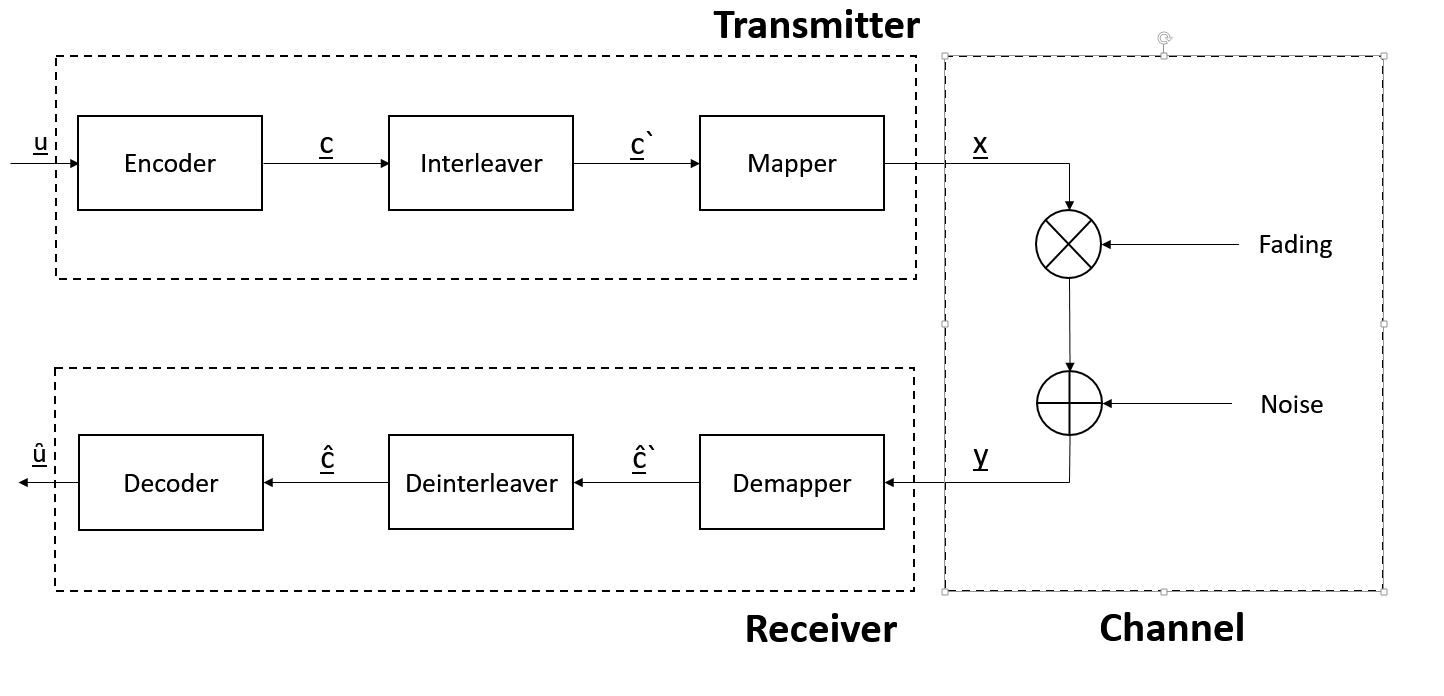
\includegraphics[width=0.95\textwidth]{Channelmodel.PNG}
	\caption{Communication chain for simulation}
	\label{fig:commchain}
\end{figure}

\section{Encoder/Decoder}
\label{sec:enc}

There are many ways to make the transmission more stable and less error prone. A major role in this protection plays the encoder and its counterpart the decoder. Encoder/decoder come in many different forms and shapes,\,e.g., as pre-built circuits in systems but more commonly today in form of coder performed as software with the help of CPUs. They reach from simple linear block codes to more complex convolutional codes to the latest turbo codes. It is also important to note, that one coder working well in \gls{AWGN} channel will often not have the same performance in a fading channel \cite[p.~262]{Goldsmith08}.
\newline
A further look will be taken into \gls{LDPC} codes, in particular the WiMax code. While \gls{LDPC} was mainly ignored in the past, since the 1999's the introduction of turbo codes and a sharp increase in computing power helped the recognition of these forms of channel coding.
\newline
\gls{LDPC} codes are linear block codes with a particular structure for their parity check matrix \textbf{H}. In the case of \gls{LDPC} codes \textbf{H} has only a small amount of nonzero entries, which means that there is a low density in the parity check matrix.
Another important difference in LDPC to turbo codes is the complexity of encoding and decoding. While turbo codes have low complexity in encoding they have high complexity in decoding. The total opposite can be said about \gls{LDPC} with high complexity in encoding and low complexity in decoding.  
\newline
WiMax, based on the IEEE 802.16 standard \cite{WiMaxTech}, is a broadband wireless technology used in small and medium distances in urban areas. It should be noted, that for WiMax codes there are predefined code lengths, code rates and encoding classes. Code lengths can range from 576 bits up to 2034 bits. Code rates are divided into four rates\footnote{$R = \frac{\textrm{number of data bits in a message}}{\textrm{number of bits in the codeword}} $}: 1/2, 2/3, 3/4, 5/6. Also the code is divided into two encoding classes A and B, which only A will be used in the simulations \cite{WIMAX}.
\newpage

\section{Bit interleaver/De-interleaver}
\label{sec:interleaver}

While the above mentioned \gls{LDPC} codes (Chapter \eref{sec:enc}) work really well on its own this is not always the case. Therefore another important block must be included in this channel. To guarantee a stable performance the method of interleaving will be introduced. Interleaving will handle a major problem in an AWGN and fading channels, namely the appearance of burst errors. In an \gls{AWGN} channel burst errors happen for modulation schemes, which assign long bit streams to a constellation symbol,\,e.g. 64-QAM. These long bit sequences can be made unrecognizable by high noise interference. In the fading channel burst errors are caused by deep fading over a set time in the transmission of the code word. \gls{LDPC} coding suffers from loss of performance trying to correct these burst errors, deteriorating even more with the increase of the burst error length. On the other hand \gls{LDPC} codes are very efficient in decoding codewords with uniformly distributed errors in the codeword. With the interleaver the code word will be shuffled into a new code word, uniformly distributing the burst errors. At the receiver a restoration of the shuffled code word back into its initial state will take place (\fig{fig:interleaver}).
\begin{figure}[!htb]
	\centering
	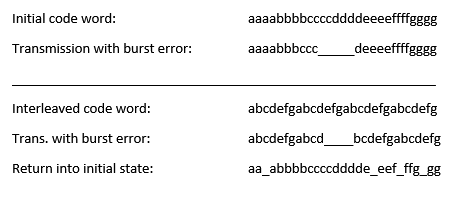
\includegraphics[width=0.8\textwidth]{interleaver.png}
	\caption{Example for interleaving}
	\label{fig:interleaver}
\end{figure}

As clearly seen in \fig{fig:interleaver} the interleaver will not remove any errors but will prevent or at least mitigate the presence of burst errors. The \gls{LDPC} decoder can correct single errors again. There are two main methods of interleaving today: symbol-interleaved coded modulation (SICM) will interleave the symbols after the modulator while \gls{BICM} will interleave the single bits before the modulator block. \gls{BICM} will be used in this thesis for having a more dominant position in practical communication systems \cite{Fabregas03}.

\clearpage

\section{Mapper/Demapper}
\label{sec:mapper}

In this block the mapper, also called the modulator, makes it possible to create a sequence of symbols out of the codeword. Group of bits are taken from the bit stream to combine them to specific constellation symbol. The symbols are located in a real/imaginary plane, also called Inphase/Quadrature planes (I/Q-planes). With the distance from the null point of the axis giving us the magnitude of the signal and the angle to the real axis the phase shift. 
\begin{figure}[!htb]
	\centering
	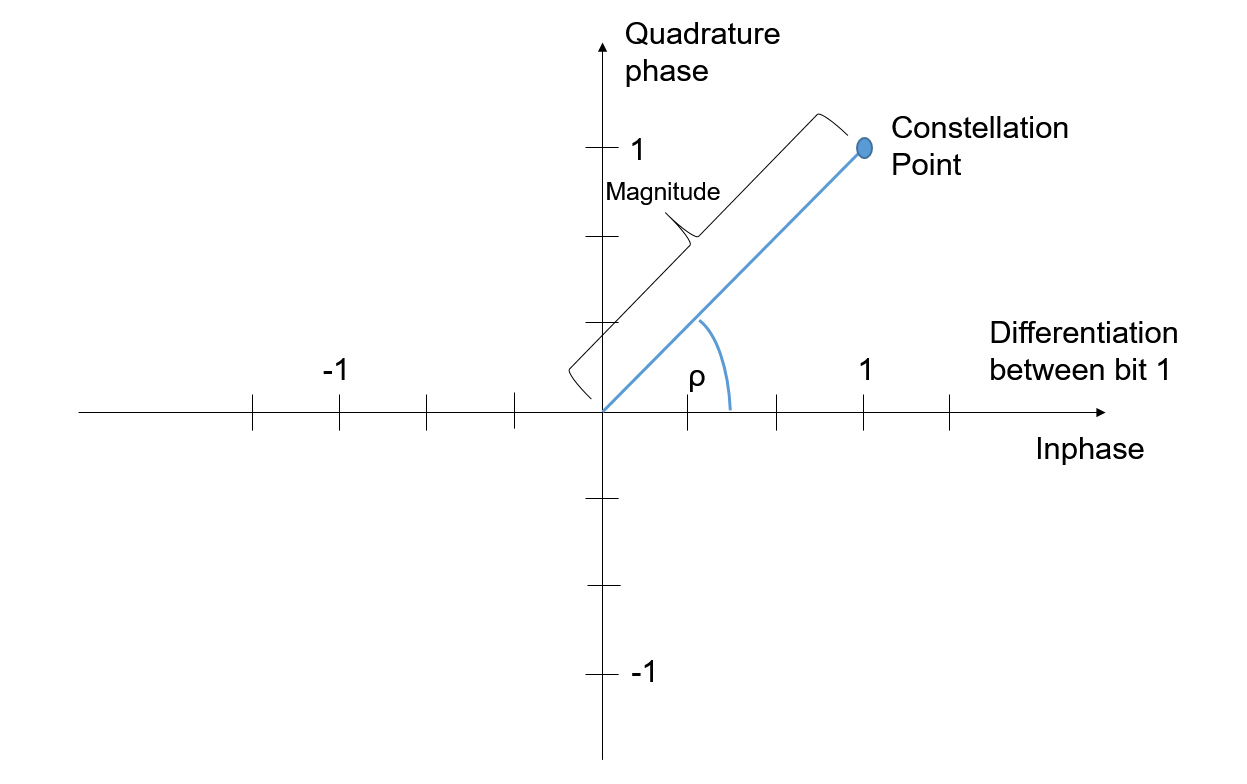
\includegraphics[width=0.8\textwidth]{IQ.png}
	\caption{Example for constellation point with amplitude and phase shift angle ($\phi$)}
	\label{fig:IQ}
\end{figure}

There are many forms of modulation schemes, with the most common ones being M-phase shift keying (PSK), M-frequency shift keying (FKS), M-amplitude modulation (AM) and M-\gls{QAM}. For the simulation, a further look will be taken at \gls{QPSK}, 16-\gls{QAM} and 64-\gls{QAM}, which are all depicted in \fig{fig:Modulation}.

\begin{figure}[!htb]
	\setlength\fwidth{0.4\textwidth}
	\setlength\fheight{0.3\textheight}
\begin{subfigure}
	
		% This file was created by matlab2tikz.
%
%The latest updates can be retrieved from
%  http://www.mathworks.com/matlabcentral/fileexchange/22022-matlab2tikz-matlab2tikz
%where you can also make suggestions and rate matlab2tikz.
%
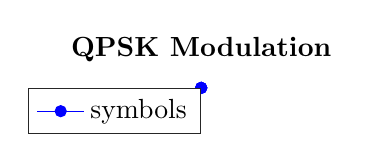
\begin{tikzpicture}

\begin{axis}[%
width=\fwidth,
height=\fheight,
at={(0\fwidth,0\fheight)},
scale only axis,
xmin=-4,
xmax=4,
xtick={-8, -7, -6, -5, -4, -3, -2, -1,  0,  1,  2,  3,  4,  5,  6,  7,  8},
xlabel style={font=\color{white!15!black}},
xlabel={I},
ymin=-4,
ymax=4,
ytick={-8, -7, -6, -5, -4, -3, -2, -1,  0,  1,  2,  3,  4,  5,  6,  7,  8},
ylabel style={font=\color{white!15!black}},
ylabel={Q},
axis background/.style={fill=white},
title style={font=\bfseries},
title={QPSK Modulation},
xmajorgrids,
ymajorgrids,
legend style={legend cell align=left, align=left, draw=white!15!black}
]
\addplot [color=blue, draw=none, mark=*, mark options={solid, blue}]
  table[row sep=crcr]{%
1	1\\
1	-1\\
-1	-1\\
-1	1\\
};
\addlegendentry{symbols}

\end{axis}
\end{tikzpicture}%
\end{subfigure}
\begin{subfigure}
	
	% This file was created by matlab2tikz.
%
%The latest updates can be retrieved from
%  http://www.mathworks.com/matlabcentral/fileexchange/22022-matlab2tikz-matlab2tikz
%where you can also make suggestions and rate matlab2tikz.
%

\begin{tikzpicture}

\begin{axis}[%
width=\fwidth,
height=\fheight,
at={(0\fwidth,0\fheight)},
scale only axis,
xmin=-4,
xmax=4,
xtick={-8, -7, -6, -5, -4, -3, -2, -1,  0,  1,  2,  3,  4,  5,  6,  7,  8},
xlabel style={font=\color{white!15!black}},
xlabel={I},
ymin=-4,
ymax=4,
ytick={-8, -7, -6, -5, -4, -3, -2, -1,  0,  1,  2,  3,  4,  5,  6,  7,  8},
ylabel style={font=\color{white!15!black}},
ylabel={Q},
axis background/.style={fill=white},
title style={font=\bfseries},
title={16-QAM Modulation},
xmajorgrids,
ymajorgrids,
legend style={at={(0.6,0.9)}, anchor=south west, legend cell align=left, align=left, draw=white!15!black}
]
\addplot [color=blue, draw=none, mark=*, mark options={solid, blue}]
  table[row sep=crcr]{%
3	3\\
3	1\\
3	-1\\
3	-3\\
1	3\\
1	1\\
1	-1\\
1	-3\\
-1	3\\
-1	1\\
-1	-1\\
-1	-3\\
-3	3\\
-3	1\\
-3	-1\\
-3	-3\\
};


\end{axis}
\end{tikzpicture}%
\end{subfigure}
\begin{subfigure}

	% This file was created by matlab2tikz.
%
%The latest updates can be retrieved from
%  http://www.mathworks.com/matlabcentral/fileexchange/22022-matlab2tikz-matlab2tikz
%where you can also make suggestions and rate matlab2tikz.
%

\begin{tikzpicture}

\begin{axis}[%
width=\fwidth,
height=\fheight,
at={(0\fwidth,0\fheight)},
scale only axis,
xmin=-8,
xmax=8,
xtick={-8, -7, -6, -5, -4, -3, -2, -1,  0,  1,  2,  3,  4,  5,  6,  7,  8},
xlabel style={font=\color{white!15!black}},
xlabel={I},
ymin=-8,
ymax=8,
ytick={-8, -7, -6, -5, -4, -3, -2, -1,  0,  1,  2,  3,  4,  5,  6,  7,  8},
ylabel style={font=\color{white!15!black}},
ylabel={Q},
axis background/.style={fill=white},
title style={font=\bfseries},
title={64-QAM Modulation},
xmajorgrids,
ymajorgrids,
legend style={at={(0.656,0.78)}, anchor=south west, legend cell align=left, align=left, draw=white!15!black}
]
\addplot [color=blue, draw=none, mark=*, mark options={solid, blue}]
  table[row sep=crcr]{%
7	7\\
7	5\\
7	3\\
7	1\\
7	-1\\
7	-3\\
7	-5\\
7	-7\\
5	7\\
5	5\\
5	3\\
5	1\\
5	-1\\
5	-3\\
5	-5\\
5	-7\\
3	7\\
3	5\\
3	3\\
3	1\\
3	-1\\
3	-3\\
3	-5\\
3	-7\\
1	7\\
1	5\\
1	3\\
1	1\\
1	-1\\
1	-3\\
1	-5\\
1	-7\\
-1	7\\
-1	5\\
-1	3\\
-1	1\\
-1	-1\\
-1	-3\\
-1	-5\\
-1	-7\\
-3	7\\
-3	5\\
-3	3\\
-3	1\\
-3	-1\\
-3	-3\\
-3	-5\\
-3	-7\\
-5	7\\
-5	5\\
-5	3\\
-5	1\\
-5	-1\\
-5	-3\\
-5	-5\\
-5	-7\\
-7	7\\
-7	5\\
-7	3\\
-7	1\\
-7	-1\\
-7	-3\\
-7	-5\\
-7	-7\\
};


\end{axis}
\end{tikzpicture}%
\end{subfigure}	
	\caption{Modulation in I/Q planes for QPSK, 16-QAM and 64-QAM}
	\label{fig:Modulation}
\end{figure}

With \gls{QPSK} the symbols all share the same amplitude and only differ in their respective phase angle. To each symbol we can assign $log2(M)$ bits, with M being the number of symbols in the scheme. Therefore, for \gls{QPSK} the number of bits per symbol amount to 2.
\newline
For 16-\gls{QAM} a maximum of 4 bits per symbols and for 64-\gls{QAM} 6 bits per symbol can be achieved. 

\clearpage

\section{Channel}
\label{sec:channel} 
The channel can be modeled in many different ways. Various sources of noise or fading can be applied, which will relate to real world interferences. Some interferences experienced in real life transmission are, e.g., thermal noise, distance fading, doppler effect and reflection of signals. To approach those kind of interferences there are many different channel models, like the \gls{AWGN} channel or Rayleigh/Rician fading. A further look in the \gls{AWGN} channel and Rayleigh fading will be given. A small graphic will further illustrate the usual culprits for degradation of signal power and resulting loss in communication performance (\fig{fig:interferences}).
\begin{figure}[!htb]
	\centering
	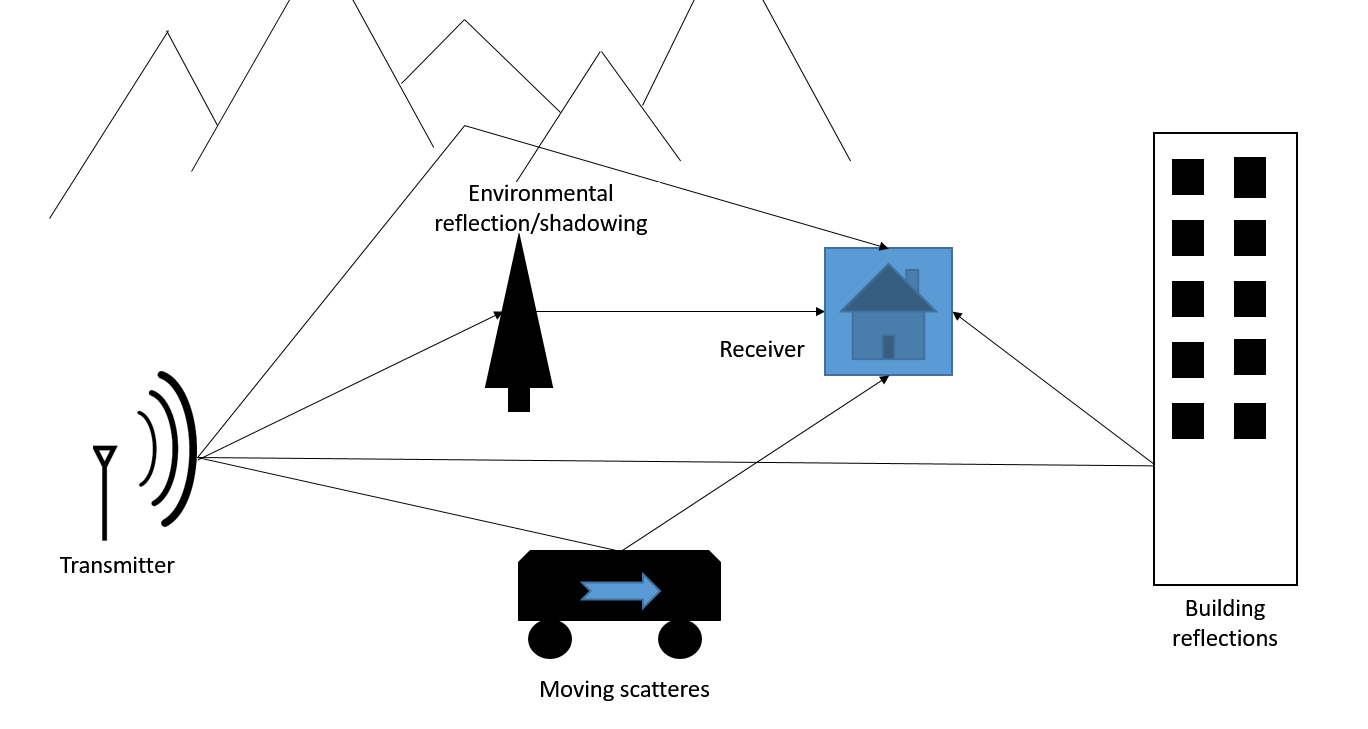
\includegraphics[width=0.95\textwidth]{reflections.png}
	\caption{Interferences in a normal transmission between two devices}
	\label{fig:interferences}
\end{figure}
\newpage
\subsection{AWGN Channel}
\label{AWGN}

The easiest kind of channel manipulation is to add random Gaussian noise to the channel, also commonly known as an \gls{AWGN} channel. Like the name says we will add noise, which is a random Gaussian distribution with flat spectral density, to an existing transmitted signal.
First of all a definition for \acrfull{SNR} is given:
\begin{equation}
\label{eq:SNR}
\textrm{SNR} = \frac{\E[{\lvert X \rvert}^2]}{\E[{\lvert N \rvert}^2]} = \frac{\sigma_{x}^2}{1},
\end{equation}
Second the probability density function of a Gaussian distribution need to be defined:
\begin{equation}
\label{eq:AWGNpdf}
P_{Y|X}(y|x) = \frac{1}{\pi\sigma^2}e^{-\frac{(y-x)^2}{\sigma^2}},  
\end{equation}
Our receiver will receive a signal like this:
\begin{equation}
\label{eq:1.1}
Y = X + N ,
\end{equation}
with Y being the received symbols, X $\sim \mathcal{N}_c(0,\sigma_{x}^2)$ the send symbol and N $\sim \mathcal{N}_c(0,1)$ the complex AWGN noise. This can be applied for a full transmission of messages resulting in:
\begin{equation}
\label{eq:1.2}
\underline{Y} = \underline{X} + \underline{N},
\end{equation}
which can be depicted more detailed like this:
\begin{equation}
\label{eq:1.3}
[Y_1,Y_2,...,Y_n] = [X_1,X_2,...,X_n] + [N_1,N_2,...,N_n],
\end{equation}
the lowercase n noting the length of the code word.
with y being the acquired point,x the transmitted symbol and $\sigma^2$ the variance of the distribution.
Gaussian noise, representing thermal noise and overlay with multiple users in a wireless system, is therefore used in all the simulations run in this thesis. In \fig{fig:AWGNSP} a depiction of the spectral power distribution of \gls{AWGN}.
\begin{figure}[!htb]
	\centering
	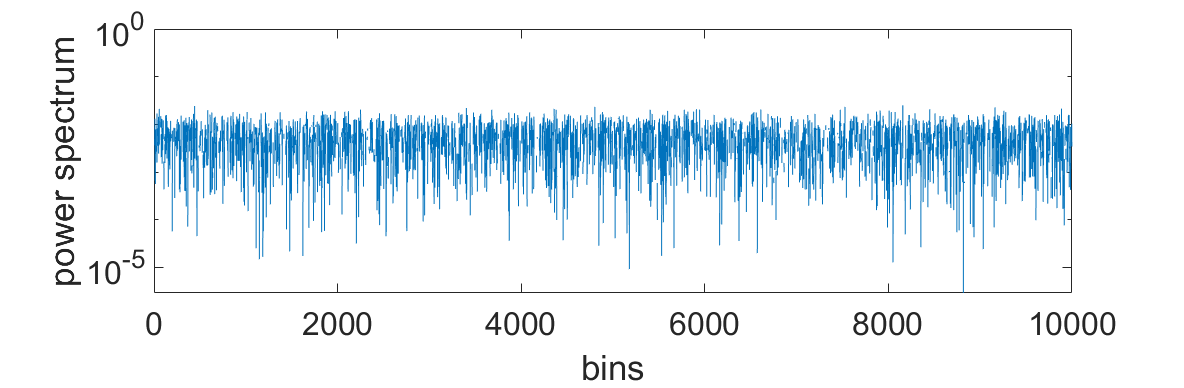
\includegraphics[width=0.95\textwidth]{AWGN.png}
	\caption{Power spectral density in a AWGN channel}
	\label{fig:AWGNSP}
\end{figure}
\newpage
\subsection{Rayleigh Fading Channel}
\label{sec:rayleigh}
Another common channel model used in communication theory is Rayleigh fading. Rayleigh fading simulates multi path reception, which means that for a receiver antenna in a wireless link there are many reflected and scattered signals reaching it (\fig{fig:interferences}). These kind of reflections are often seen in high-density urban areas. This results in construction or destruction of signal waves. The channel will now look like this:
\begin{equation}
\label{eq:rayleigh1}
Y = HX + N,  
\end{equation}
which adds the new fading coefficient H to the transmitted message.
\newline
As shown before in the \gls{AWGN} channel the above \eq{eq:rayleigh1} can be expanded for a full transmission. Before that it needs to be clarified that not every symbol will be multiplied with a different fading coefficient H, but a whole block of symbols. This kind of transmission with Rayleigh fading is known as block fading:
\begin{equation}
\label{eq:rayleigh2}
[Y_1,...,Y_{kT}] = [H_1X_1,...,H_1X_T]...[H_kX_{(K-1)T+1},...,H_kX_{kT}] + [N_1,...,N_{kT}] \textrm{ , } kt = n,  
\end{equation}
with the subscript $T$ indicating the length of the block, $k$ the number of blocks in a codeword and $n$ the length of the codeword. The block length can be chosen ranging from on single symbol up to the whole code word being one block.
\newline
The graphic (\fig{fig:rayleigh}) shows the power distribution over 12000 samples. Being Gaussian randomly distributed there are now these so called "deep fadings" where the power of the fading drops, which will also decrease the signal power of the received signal to drop significantly. This results in the so-called burst errors, which were mentioned in Chapter \eref{sec:interleaver}.
\begin{figure}[!htb]
	\centering
	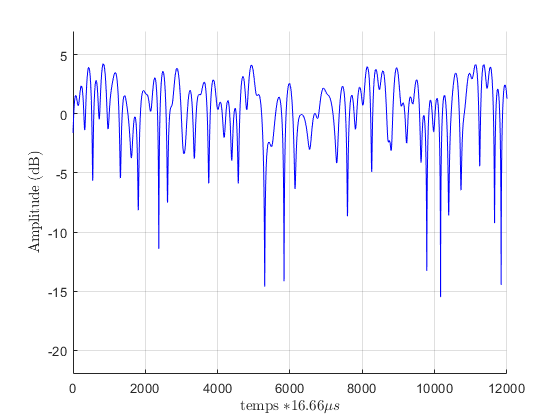
\includegraphics[width=0.95\textwidth]{rayleigh.png}
	\caption{Power spectral density in a Rayleigh channel}
	\label{fig:rayleigh}
\end{figure}  % Include introduction / Einbinden des Kapitels Einleitung/Problemstellung
        %%%%%%%%%%%%%%%%%%%%%%%%%%%%%%%%%%%%%%%%%%%%%%
\chapter{Capacity in AWGN Channel} \label{chap:awgnchan}
%%%%%%%%%%%%%%%%%%%%%%%%%%%%%%%%%%%%%%%%%%%%%%%
\graphicspath{{C:/Users/Kevin/Bachelarbeit/Bachelorarbeit/01_Bachelorarbeit_LaTex/02_Figures/}}

In this section we will discuss the capacity of a wireless channel with \gls{AWGN} noise interfering with the transmission between transmitter and receiver. 
\newline
In general, capacity \textit{C} can be defined as the maximum data rate \textit{R} at which information can be reliably transmitted over a channel, that means the highest rate of transmission with a very low error probability rate. It is proven that any rate exceeding the maximum capacity rate of the channel will result in error rates deviating from zero \cite{Shannon}. In modern technology with the help of smart modulation schemes and coding methods a rate close to the capacity can be achieved.
All the capacities in the following simulations will be for complex and time-discrete channels. 
While time-continuous systems are analyzed for real world applications, most systems can be converted into a time-discrete model with same capacity results \cite{Goldsmith08}. 
\section{Capacity and Monte-Carlo-Simulation}
\label{sec:capAWGN}

For a \gls{AWGN}-Channel the simple channel model already defined in \eq{eq:1.1} will be used:
\begin{equation}
\label{eq:chanAWGN}
Y = X + N,   
\end{equation}
with X $\sim \mathcal{N}_c(0,{\sigma_{x}}^2$) and N $\sim \mathcal{N}_c(0,1)$. The received signal Y will have a distribution of \mbox{Y $\sim \mathcal{N}_c(0,{\sigma_{x}}^2+1$)} under the condition that X and N being independently distributed.
Now the capacity as a maximum of mutual information I between X and Y will be calculated, with X and Y being two independent randomly normal distributed variables.
\newline
For the mutual information further calculations will lead to the differential entropy:
\begin{equation}
I(X;Y) = h(Y) - h(Y|X)
= h(Y) - h(N),
\end{equation}
with N also being independent from X.
\newline
This further simplifies to 
\begin{equation}
h(Y) = h(X+N) = log(\pi e^{\sigma^2+1}) \quad \textrm{and} \quad h(Y|X) = h(N) = log(\pi e^{1}),
\end{equation}
which will lead us to the final equation for the capacity in an AWGN-channel:
\begin{equation}
\label{eq:AWGNcap}
C = log(1+\sigma^2),
\end{equation}
as proved in \cite{Kramer}.
\newline
With this approach a good approximation of values for further calculations with added modulation schemes has been given. The above calculated data rate can be used as upper bound for any further capacity calculation done, this means there should be no capacity rate, especially for real world applications, exceeding this capacity rate \cite{Shannon}.


\section{Capacity for QPSK and M-QAM}
Now the capacity will be calculated for the three above mentioned modulation schemes (Chapter \eref{sec:mapper}). The schemes will be plotted with the capacity calculations for the Gaussian channel to give us a overall comparison and overview.
\newline
Before the simulation or any calculation is done it can already be assumed how QPSK will behave for high SNR. As stated before QPSK (Chapter \eref{sec:mapper}) can transmit up to 2 bits per symbol. So the plot will approach the 2 bit per symbol border for high SNR. The same assumption can be applied to both 16-QAM and 64-QAM.
After creating a random codeword modulated with the fitting modulation scheme, noise is added to the signal, which is then received as the bit stream Y. The next step is to calculate the capacity. 
\newline
Starting with the mutual information again we get:
\begin{equation}
I(X_Q;Y) = h(Y) - h(Y|X_Q) = h(Y) - h(N).
\end{equation}
Now the differential entropy for h(Y) has to be calculated: 
\begin{equation}
\label{eq:MCEntropy}
h(Y) = {\E}_Y[-log(p_Y(y)]
\end{equation}
Applying the Monte-Carlo-Simulation will simplify the calculation giving us the expected value of the \eq{eq:MCEntropy}. The Monte-Carlo-Simulation will be further explained in the following chapter (Ch. \ref{sec:MCS}).
\begin{equation}
\label{eq:entropy1}
h(Y) =  \frac{1}{N}\sum_{i=0}^N(-log(p(y\textsubscript{i}))),
\end{equation} 
Now $p_Y(y)$ has to be calculated. $P_Y(y)$ takes in consideration the possible input and output pairs $x \in X$ and $y \in Y$. The sum over all these pairs is taken:
\begin{equation}
\label{eq:entropy2.1}
p_Y(y) = \sum_{n=1}^{k}p_{Y|X}(y|x)p_X(x) = \frac{1}{k}\sum_{n=1}^{k}p_{Y|X}(y|x), 
\end{equation}
with $p_{Y|X}(y|x)$ already defined in \eq{eq:AWGNpdf} 
\begin{equation}
\label{eq:entropy2}
p_Y(y) = \frac{1}{k}*\sum_{n=1}^{k}\frac{1}{\pi}(e^{y-x\textsubscript{n}}),
\end{equation} 
with x being the constellation points and y the received symbol.
Here we only need to watch out for the number of symbols in the modulation scheme. For QPSK we have a \mbox{k = 4}, 16-QAM a k = 16 and 64-QAM a k = 64.
\newline
\subsection{Monte-Carlo-Simulation}
\label{sec:MCS}
Monte Carlo Simulation is widely used in stochastic to get solutions for random experiments. It is applied to solve analytical unsolvable problems numerically. MC is based upon the law of large numbers, which says that a large number of performing the same random experiment will lead the average of the results close to the expected value[Cite Law of Random Numbers!]. 
Applied to \eq{eq:MCEntropy}:
\begin{equation}
\label{eq:MCEntropy2}
h(Y) = {\E}_Y[f(y)],
\end{equation}
with $f(y) = -log(p_Y(y))$. So we want to calculate the expected value from our function $f(y)$. 
\newline
Applying \gls{MC} with $N$ sample size:
\begin{equation}
\frac{1}{N}\sum_{i=1}^{N}f(y_i) 
\end{equation}
which after \gls{MC} equals to the expected value of our function $f(y)$.
\begin{equation}
\frac{1}{N}\sum_{i=1}^{N}f(y_i) = \E_Y[f(y)],
\end{equation}
which is also the answer for the initial \eq{eq:MCEntropy}.
We take this as a base to get reliable results. The Monte Carlo simulations will be used for two calculations, once already used above for calculating the differential entropy and later once to calculate a theoretical Rayleigh fading curve out of the AWGN channel. 

\subsection{Implementation in MATLAB}
\label{AWGNMAT}
We now implement the mentioned \eq{eq:entropy1} and \eref{eq:entropy2} in MATLAB and plot the results. The code has to take into consideration the modulation schemes used, the range of calculation (SNR range\footnote{SNR range is the difference between lowest SNR value to highest SNR value}) and the sample size N. The code runs through the SNR range, here ranging from -10\,dB to 30\,dB in step sizes of 0.5\,dB. The sample size N also has to be large enough to apply the Monte-Carlo simulation reliably. In our simulation N has to be higher than 10000 samples to receive reliable results. First a random bit stream, functioning as the data, is initialized. The bit stream is passed through a modulator which assigns the corresponding symbol. We scale the created constellation point with the SNR value. After passing \underline{X} through the complex AWGN channel the resulting symbols \underline{Y} and \underline{X} are put into \eq{eq:entropy1} and \eref{eq:entropy2}. Done for every step size a resulting plot for the capacity over SNR is created.  
    

\section{Results}
\begin{figure}[!htb]
		\setlength\fwidth{0.8\textwidth}
	\setlength\fheight{0.4\textheight}
	\centering
	% This file was created by matlab2tikz.
%
%The latest updates can be retrieved from
%  http://www.mathworks.com/matlabcentral/fileexchange/22022-matlab2tikz-matlab2tikz
%where you can also make suggestions and rate matlab2tikz.
%
\definecolor{mycolor1}{rgb}{0.00000,0.44700,0.74100}%
\definecolor{mycolor2}{rgb}{0.85000,0.32500,0.09800}%
\definecolor{mycolor3}{rgb}{0.92900,0.69400,0.12500}%
\definecolor{mycolor4}{rgb}{0.49400,0.18400,0.55600}%
%
\begin{tikzpicture}

\begin{axis}[%
width=0.951\fwidth,
height=\fheight,
at={(0\fwidth,0\fheight)},
scale only axis,
xmin=-10,
xmax=30,
xlabel style={font=\color{white!15!black}},
xlabel={SNR in dB},
ymin=0,
ymax=8,
ylabel style={font=\color{white!15!black}},
ylabel={Bits per Symbol},
axis background/.style={fill=white},
title style={font=\bfseries},
title={Capacity of different Modulation Schemes},
xmajorgrids,
ymajorgrids,
legend style={at={(0.1,0.74)}, anchor=south west, legend cell align=left, align=left, draw=white!15!black}
]
\addplot [color=mycolor1, line width=1.5pt]
  table[row sep=crcr]{%
-10	0.137503523749935\\
-9	0.171069138514397\\
-8	0.212244743260396\\
-7	0.262464707140879\\
-6	0.323299322693842\\
-5	0.396409161163113\\
-4	0.483474953345681\\
-3	0.586103926445347\\
-2	0.705719050773514\\
-1	0.843443825203654\\
0	1\\
1	1.17563663469239\\
2	1.37010466975099\\
3	1.58268235491156\\
4	1.81224619130063\\
5	2.05737320860679\\
6	2.31645617962626\\
7	2.58781437356203\\
8	2.86978721917028\\
9	3.16080442391302\\
10	3.4594316186373\\
11	3.76439436704286\\
12	4.07458523490543\\
13	4.38905896736305\\
15	5.02780767335052\\
17	5.67577990180488\\
19	6.32971245944191\\
22	7.31731600193655\\
25	8.30937524121281\\
};
\addlegendentry{Gaussian}

\addplot [color=mycolor2, line width=1.5pt]
  table[row sep=crcr]{%
-10	0.134318676891414\\
-9	0.174635816483672\\
-8	0.20485508504726\\
-6	0.327039186611294\\
-4	0.472082307912629\\
-3	0.573554328684857\\
-2	0.697612166121157\\
-1	0.825758566915063\\
0	0.97722496808991\\
1	1.12117023488211\\
2	1.29655560298805\\
3	1.44560427893327\\
4	1.58287550462634\\
5	1.72395861932077\\
6	1.81975490754443\\
7	1.9009265237288\\
8	1.95124512760905\\
9	1.97900262101901\\
10	1.99726464467178\\
11	1.99465702352565\\
13	2.00621645432518\\
14	1.99775717802409\\
15	1.99352324063785\\
16	1.99288352080239\\
17	2.00569199393895\\
18	1.99417788919495\\
19	2.00093573257148\\
20	1.99323614943762\\
21	2.0023569582242\\
22	2.00055808362006\\
23	2.00349870239276\\
24	1.99248898600768\\
25	2.00581283635647\\
26	2.00900754557807\\
27	2.00264928435469\\
28	2.00303909608031\\
29	2.0065941140835\\
30	1.99779049448823\\
};
\addlegendentry{QPSK}

\addplot [color=mycolor3, line width=1.5pt]
  table[row sep=crcr]{%
-10	0.133078621094946\\
-9	0.173494547979338\\
-8	0.220908856165408\\
-7	0.264478176941324\\
-6	0.334954581192878\\
-5	0.395599356878865\\
-4	0.484286286618719\\
-2	0.718644217026682\\
-1	0.852487246141862\\
0	1.00829230213079\\
2	1.35874349552977\\
3	1.55736333860045\\
4	1.76872449143159\\
6	2.21865411768635\\
7	2.45352460795739\\
8	2.6999684486276\\
9	2.94200816606406\\
10	3.17169835013319\\
11	3.3914410424218\\
12	3.57981844984042\\
13	3.73829824505448\\
14	3.85167389656089\\
15	3.93507122701873\\
16	3.96957657428747\\
17	3.99106448779695\\
19	4.00430286417342\\
20	4.00090932752551\\
21	3.99085339568459\\
22	4.00890643100917\\
23	4.00164450497164\\
24	3.99853300031333\\
25	3.99141345784766\\
26	4.00344520032089\\
27	3.99874218725454\\
28	3.9977577896723\\
30	4.00292705817962\\
};
\addlegendentry{16-QAM}

\addplot [color=mycolor4, line width=1.5pt]
  table[row sep=crcr]{%
-10	0.134850667838428\\
-9	0.172617267320625\\
-8	0.203316768228184\\
-6	0.31285660634952\\
-4	0.470750556735766\\
-3	0.569780003901307\\
-2	0.69120016442837\\
-1	0.824570100925076\\
0	0.978787118586471\\
1	1.14983050695955\\
2	1.33668838474587\\
3	1.53140347948951\\
4	1.7432857972603\\
5	1.97220315303569\\
7	2.45903091869015\\
8	2.72341635331581\\
9	2.98208659021222\\
10	3.25360041031622\\
12	3.80643855049868\\
13	4.10274121811894\\
14	4.38342550056116\\
16	4.9537936278703\\
17	5.22045607641617\\
18	5.4574450375468\\
19	5.65544704188428\\
20	5.79766176488834\\
21	5.89716313853225\\
22	5.94925122298661\\
23	5.98186058528657\\
24	5.99629634168651\\
26	5.99453237495413\\
27	5.99881714560789\\
28	5.9955600103224\\
30	5.99773926484703\\
};
\addlegendentry{64-QAM}

\end{axis}
\end{tikzpicture}%
	\caption{Capacity plot for general AWGN-channel, QPSK, 16-QAM and 64-QAM}
	\label{fig:capmod}
\end{figure}
The results of all the \gls{MC} for all the modulation schemes done in MATLAB are presented in \fig{fig:capmod}. The plot shows the capacity for a simple Gaussian channel and the three modulation schemes mentioned in Chapter \eqref{sec:mapper}. We plot the resulting capacity calculated over the corresponding SNR values. 
It can be seen that for all three modulation schemes that for higher \gls{SNR} they will approach the expected maximum number of bits per symbol. For \gls{QPSK} to reach the maximum bit rate a \gls{SNR} of about 7.5\,db is needed. Similarly 16-QAM needs 15\,dB and 64-QAM 22\,dB. 
\newline
Also the Gaussian distributed codeword clearly outperforms the modulated codeword, especially  after 0\,dB SNR. As already discussed before the Gaussian capacity is the upper bound with no modulation exceeding it the following results and plot can confirm the validity of the simulation.


\clearpage
        %%%%%%%%%%%%%%%%%%%%%%%%%%%%%%%%%%%%%%%%%%%%%%%
\chapter{Frame Error Rate for AWGN Channel}
 \label{chap:AWGN chain}
%%%%%%%%%%%%%%%%%%%%%%%%%%%%%%%%%%%%%%%%%%%%%%%
\graphicspath{{C:/Users/Kevin/Bachelarbeit/Bachelorarbeit/01_Bachelorarbeit_LaTex/02_Figures/}}

This section will further built upon the topics discussed in the previous chapters. We will now build a communication chain using the blocks discussed in Chapter 2. After the transmission the \gls{FER} will be determined. The \gls{FER} is the estimated rate of faulty transmissions in one whole simulation. We will be sending frames of code words each consisting of 576 up to 2048 bits. After comparison between the sent code word and the decoded code word at the receiver we determine a frame error. If the decoded codeword has any wrong bit the whole frame will be marked as a faulty frame. This will be done for a certain amount of frames.

\section{LDPC and the Coded Modulation Library}
Already explained in Chapter 1 the whole transmission will be done with the coding method of \gls{LDPC}. For the coding and decoding we will be using the Coded Modulation Library. This library and the functions used in this simulation will be further explained now.
\newline
The Iterative Solutions Coded Modulation Library (ISCML) is an open source toolbox for simulating capacity approaching codes in MATLAB\cite{CML}. The toolbox supports many different standard linear block codes and turbo codes. With many of the complex and computational heavy codes implemented in C and ported back to MATLAB as so called C-mex functions\cite{CML}.
\newline 
For this thesis a further look will be taken at the WiMax LDPC code. The coder function will create the parity-check-matrix \textbf{H} with a given code word length $n$ and rate $r$. The code word which will be sent will be created like this:
\begin{equation}
\label{eq:LDPC1}
\boldmath{H}*a^T = 0,
\end{equation}
with $a$ being the code word transmitted. Further noted $a$ consists of the relevant data $a_{d}$, which is known, and the unknown check nodes $a_{r}$. 
\begin{equation}
\label{eq:LDPC2}
a_r = (\boldmath{H}_k)^{-1} * H_l * a_n
\end{equation}
The decoding will also be done by the \gls{CML} which again uses the parity-check matrix \textbf{H}. The received code word has to fulfill this condition:
\begin{equation}
\label{eq:LDPC3}
\boldmath{H}*b^T = 0,
\end{equation}
with $b^T$ being the received code word. This will be checked with typical graph solving algorithms. For LDPC the commonly used algorithm is the sum-product algorithm.
With the \gls{CML} the first and last block of the full communication chain (\fig{fig:commchain}) is implemented.
\section{Demapping after AWGN}
Another big part of a functioning communication chain is the estimation of the code word from the received symbol stream $\boldmath\underline{Y}$, which passed the channel experiencing various kind of noises and fadings. There are two main forms of restoring the code word, namely hard-decision demapping and soft-decision demapping.
\subsection{Hard-Decision Demapping vs. Soft-Decision Demapping}
We will now discuss the benefits between hard-decision and soft-decision demapping. Hard-decision demapping makes a decision based on the decision boundary of the received symbol. While soft demapping will take into consideration all symbol constellations in the modulation scheme.
It is proven that soft demapping will achieve better demapping results while hard demapping is not as complex as soft demapping \cite{GaussianWaves}.In our case we do not mind a complex system which takes more time but are more focused on achieving the maximum rate of successful transmissions.
\newpage
\subsection{Log-Likelihood Ratio}
A soft demapper will now be implemented in this system. The soft demapper will result in turning the symbols in the corresponding bit block.
\begin{figure}[!htb]
    \centering
    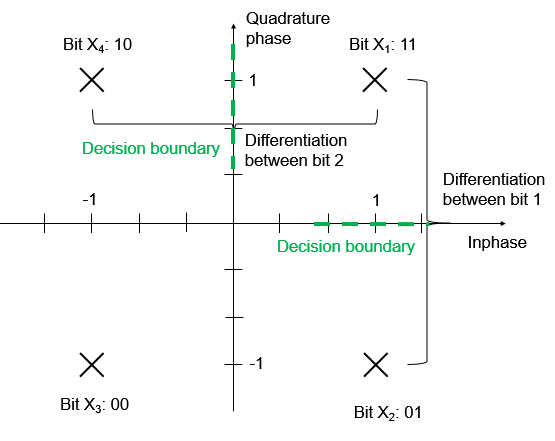
\includegraphics[width=0.8\textwidth]{llr.png}
    \caption{Depiction of soft demapper in I/Q-plane}
    \label{fig:llr}
\end{figure}
\newline
As seen in the figure above we have a \gls{QPSK} modulated codeword. Symbols \textbf{\underline{Y}} received can be located anywhere on the I/Q-plane distorted by AWGN. We will now assume a single symbol $Y$ received at the demapper.
With QPSK consisting of two bit blocks $[B_1B_2]$ first a differentiation for the first bit is done.
\begin{equation}
\label{eq:llr1}
L^n = log\frac{P(B_1=0|Y)}{P(B_1=0|Y)}
\end{equation}
With Baye's rule:
\begin{equation}
\label{eq:bl}
P(B_1=0|Y) = \frac{P(Y|B_1=0)}{p(Y)}*P(Y=0),
\end{equation}
the equation simplifies to 
\begin{equation}
L^n = log\frac{P(Y|B_1=0)}{P(Y|B_1=1)},
\end{equation}
with $P(Y=0)=P(Y=1)=0.5$.
Getting back to \fig{fig:llr} it can be determined that $X_1$ and $X_4$ have $B_1=1$ while $X_2$ and $X_3$ result in $B_1=0$.
\begin{equation}
L^n = log\frac{P(Y|X_2)+P(Y|X_3)}{P(Y|X_1)+P(Y|X_4)}.
\end{equation}
With \eq{eq:AWGNpdf} the log likelihood for bit $B_1$ can now be calculated. The corresponding bit $B_2$ will also be determined like this. In the end a code word is received as log likelihood ratios\cite{SoftDemapping}.
\section{FER}
\label{sec:FER}
The \gls{FER} can now be determined with the help of the two previous sections. By dividing the number of faulty frames from the total number of frames we get the \gls{FER}. It should be noted that not every \gls{FER} calculated is a reliable result for our simulation. For a whole simulation run a certain amount of faulty frames is needed, usually at least 50 faulty frames need to be detected. It can be seen like this: A simulation run for 100 frames with 1 faulty frame does not give a confident result of a \gls{FER} of 0.01. While a simulation ran for 10000 frames with 100 faulty frames will be seen as a more reliable result for a \gls{FER} of 0.01. 
\newline
With the proposition above for a \gls{FER} of $10^{-4}$ we would need to run a simulation with $10^6$ frames. Now the problem of simulation time length arises. If lower \gls{FER} needs to be calculated the number of frames will rise. Also while maybe feasible for short SNR ranges some calculations will need longer SNR-ranges, which becomes a problem in the further chapters for fading channels. Both combined will make the simulation run rather long.
\newline
Two methods to reduce the simulation time are now implemented: The first one being a premature break of the simulation after reaching 100 faulty frames and dividing by the number of iterations ran. Even if running the whole simulation resulting in more precise \gls{FER}, 100 faulty frames are enough for plotting a reliable result. Another technique is to increase the step size of the SNR between simulations, which will allow us to keep the SNR range at the expense of plot resolution. This can be mitigated by interpolating the results, which means we numerically create more data samples to increase the plot resolution.

\newpage
\section{Simulation Results}
All the above discussed methods are implemented in MATLAB.
The simulation will be run for an SNR range of 0\,dB-10\,dB SNR. Furthermore a \gls{FER} of at least $10^{-3}$ should be calculated, which is a total of 10000 frames run. The following plot shows the \gls{FER} plots for all three modulation schemes.
Now with the  \gls{FER} calculated the capacity plots from chapter \eref{chap:awgnchan} can be used again for comparison. In this part the FER calculation are used by examining the interpolated data. Setting a threshold at $10^{-3}$ FER the corresponding SNR value is noted down. The value is then plotted into the capacity plot. It has to be taken into account the rate of \gls{LDPC} coding used. The rate defines the amount of relevant data in a whole frame/code word. That means for a rate of $1/2$ the transmission of relevant data is halved. For QPSK with a maximum of 2 bits per symbols and a rate of $1/2$ a information value of only 1 bit per symbol can be achieved.
\newline
\begin{figure}[!htb]
	\setlength\fwidth{0.9\textwidth}
	\setlength\fheight{0.4\textheight}
	\centering
	% This file was created by matlab2tikz.
%
%The latest updates can be retrieved from
%  http://www.mathworks.com/matlabcentral/fileexchange/22022-matlab2tikz-matlab2tikz
%where you can also make suggestions and rate matlab2tikz.
%
\definecolor{mycolor1}{rgb}{0.00000,0.44700,0.74100}%
\definecolor{mycolor2}{rgb}{0.74902,0.00000,0.74902}%
\definecolor{mycolor3}{rgb}{0.85098,0.32549,0.09804}%
\definecolor{mycolor4}{rgb}{0.46667,0.67451,0.18824}%
%
\begin{tikzpicture}

\begin{axis}[%
width=0.951\fwidth,
height=\fheight,
at={(0\fwidth,0\fheight)},
scale only axis,
xmin=-5,
xmax=25,
xlabel style={font=\color{white!15!black}},
xlabel={SNR in dB},
ymin=0,
ymax=2.5,
ylabel style={font=\color{white!15!black}},
ylabel={Bits per symbol},
axis background/.style={fill=white},
title style={font=\bfseries},
title={FER (0.001) of QPSK with Gaussian Noise},
xmajorgrids,
ymajorgrids,
legend style={at={(0.05,0.65)}, anchor=south west, legend cell align=left, align=left, draw=white!15!black}
]
\addplot [color=mycolor1, line width=1.5pt]
  table[row sep=crcr]{%
-6	0.323068206330696\\
-5	0.391326071720055\\
-4	0.48489476841884\\
-3	0.574809791357794\\
-2	0.698200176432383\\
-1	0.833818491736498\\
0	0.972778527481442\\
1	1.12495846691126\\
2	1.28072065748154\\
3	1.44250305591488\\
4	1.58596017892716\\
5	1.722479934533\\
6	1.82567644583971\\
7	1.89431417542903\\
8	1.95776065265052\\
9	1.98017610381626\\
10	1.99433936158288\\
11	1.99258273944893\\
12	2.00345231173243\\
13	1.99904308404509\\
14	1.99922794452327\\
15	2.00370158206796\\
16	2.00276837542221\\
17	1.99652877120277\\
18	1.99843303166521\\
19	1.9989850606081\\
20	2.00488508312673\\
21	1.98995611336795\\
22	2.00455104085159\\
23	1.99686202453218\\
24	1.99923283598126\\
25	1.99341493446232\\
26	2.00059528376659\\
};
\addlegendentry{QPSK}

\addplot [color=blue, draw=none, mark size=5.0pt, line width = 1.0pt, mark=asterisk, mark options={solid, blue}]
  table[row sep=crcr]{%
1.9841	1\\
};
\addlegendentry{R = 1/2}

\addplot [color=mycolor2, draw=none, mark size=5.0pt, line width = 1.0pt, mark=asterisk, mark options={solid, mycolor2}]
  table[row sep=crcr]{%
3.9409	1.33333333333333\\
};
\addlegendentry{R = 2/3}
\addplot [color=mycolor3, draw=none, mark size=5.0pt, line width = 1.0pt, mark=asterisk, mark options={solid, mycolor3}]
  table[row sep=crcr]{%
4.9859	1.5\\
};
\addlegendentry{R = 3/4}
\addplot [color=mycolor4, draw=none, mark size=5.0pt, line width = 1.0pt, mark=asterisk, mark options={solid, mycolor4}]
  table[row sep=crcr]{%
5.991	1.66666666666667\\
};
\addlegendentry{R = 5/6}
\end{axis}
\end{tikzpicture}%
	\caption{Capacity to FER comparison for QPSK}
	\label{fig:llr1}
\end{figure}
\begin{figure}[!htb]
	\setlength\fwidth{0.9\textwidth}
	\setlength\fheight{0.4\textheight}	
	\centering
	% This file was created by matlab2tikz.
%
%The latest updates can be retrieved from
%  http://www.mathworks.com/matlabcentral/fileexchange/22022-matlab2tikz-matlab2tikz
%where you can also make suggestions and rate matlab2tikz.
%
\definecolor{mycolor1}{rgb}{0.00000,0.44700,0.74100}%
\definecolor{mycolor2}{rgb}{0.74902,0.00000,0.74902}%
\definecolor{mycolor3}{rgb}{0.85098,0.32549,0.09804}%
\definecolor{mycolor4}{rgb}{0.00000,0.49804,0.00000}%
%
\begin{tikzpicture}

\begin{axis}[%
width=0.951\fwidth,
height=\fheight,
at={(0\fwidth,0\fheight)},
scale only axis,
xmin=-5,
xmax=25,
xlabel style={font=\color{white!15!black}},
xlabel={SNR in dB},
ymin=0,
ymax=4.5,
ylabel style={font=\color{white!15!black}},
ylabel={Bits per symbol},
axis background/.style={fill=white},
title style={font=\bfseries},
title={FER (0.001) of QAM16 with Gaussian Noise},
xmajorgrids,
ymajorgrids,
legend style={at={(0.1,0.55)}, anchor=south west, legend cell align=left, align=left, draw=white!15!black}
]
\addplot [color=mycolor1, line width=1.5pt]
  table[row sep=crcr]{%
-6	0.328621714082722\\
-5	0.410274595889064\\
-4	0.497750186881902\\
-3	0.599712705644915\\
-2	0.714042374792633\\
-1	0.861837472466473\\
0	1.00371041314962\\
1	1.17925231331639\\
2	1.36317896763643\\
3	1.56645355738085\\
5	1.9914221739593\\
6	2.22277316719511\\
7	2.45551845122164\\
8	2.70357747937736\\
9	2.93827693641367\\
10	3.18009610376135\\
11	3.38994681065897\\
12	3.57915476353915\\
13	3.73698103166151\\
14	3.85191363323502\\
15	3.93083271031978\\
16	3.98124687547666\\
17	3.98873587025561\\
18	3.9999092584337\\
19	3.99126898886324\\
20	4.00461627105919\\
22	3.99570005449973\\
23	4.00385440769931\\
24	3.99872083361317\\
25	4.0013615285833\\
26	3.99772619520965\\
};
\addlegendentry{QAM-16}

\addplot [color=blue, draw=none, mark size=5.0pt, line width = 1.0pt, mark=asterisk, mark options={solid, blue}]
  table[row sep=crcr]{%
8.4925	2\\
};
\addlegendentry{R = 1/2}

\addplot [color=mycolor2, draw=none, mark size=5.0pt, line width = 1.0pt, mark=asterisk, mark options={solid, mycolor2}]
  table[row sep=crcr]{%
10.94	2.66666666666667\\
};
\addlegendentry{R = 2/3}

\addplot [color=mycolor3, draw=none, mark size=5.0pt, line width = 1.0pt, mark=asterisk, mark options={solid, mycolor3}]
  table[row sep=crcr]{%
11.9828	3\\
};
\addlegendentry{R = 3/4}

\addplot [color=mycolor4, draw=none, mark size=5.0pt, line width = 1.0pt, mark=asterisk, mark options={solid, mycolor4}]
  table[row sep=crcr]{%
12.9956	3.33333333333333\\
};
\addlegendentry{R = 5/6}

\end{axis}
\end{tikzpicture}%
	\caption{Capacity to FER comparison for 16-QAM}
	\label{fig:llr2}
\end{figure}
\begin{figure}[!h]
	\setlength\fwidth{0.9\textwidth}
	\setlength\fheight{0.4\textheight}
	\centering
	% This file was created by matlab2tikz.
%
%The latest updates can be retrieved from
%  http://www.mathworks.com/matlabcentral/fileexchange/22022-matlab2tikz-matlab2tikz
%where you can also make suggestions and rate matlab2tikz.
%
\definecolor{mycolor1}{rgb}{0.00000,0.44700,0.74100}%
\definecolor{mycolor2}{rgb}{0.74902,0.00000,0.74902}%
\definecolor{mycolor3}{rgb}{0.85098,0.32549,0.09804}%
\definecolor{mycolor4}{rgb}{0.46667,0.67451,0.18824}%
%
\begin{tikzpicture}

\begin{axis}[%
width=0.951\fwidth,
height=\fheight,
at={(0\fwidth,0\fheight)},
scale only axis,
xmin=0,
xmax=30,
xlabel style={font=\color{white!15!black}},
xlabel={SNR in dB},
ymin=0,
ymax=6.5,
ylabel style={font=\color{white!15!black}},
ylabel={Bits per symbol},
axis background/.style={fill=white},
title style={font=\bfseries},
title={FER (0.001) of QAM64 with Gaussian Noise},
xmajorgrids,
ymajorgrids,
legend style={at={(0.1,0.55)}, anchor=south west, legend cell align=left, align=left, draw=white!15!black}
]
\addplot [color=mycolor1, line width=1.5pt]
  table[row sep=crcr]{%
-1	0.83078278973122\\
0	0.979654599592624\\
1	1.14834131414807\\
2	1.33127288676911\\
4	1.74508866458763\\
5	1.96566337984369\\
6	2.21403226346695\\
7	2.45940311575263\\
8	2.71491729771481\\
10	3.24616258413947\\
13	4.09660026502285\\
14	4.38419050112642\\
15	4.67504652219285\\
16	4.95776784876414\\
17	5.22003469749198\\
18	5.45597897518436\\
19	5.65235382550127\\
20	5.79883674591287\\
21	5.89932124254842\\
22	5.95960529647478\\
23	5.98793504239796\\
24	5.99162626739952\\
25	6.00358017470219\\
26	5.99555782274282\\
27	5.99166132276335\\
28	5.99097580881566\\
29	6.00114495777247\\
30	5.98912057361096\\
31	6.00260416766955\\
};
\addlegendentry{QAM-64}

\addplot [color=blue, draw=none, mark size=5.0pt, line width = 1.0pt, mark=asterisk, mark options={solid, blue}]
  table[row sep=crcr]{%
14.4588	3\\
};
\addlegendentry{R = 1/2}

\addplot [color=mycolor2, draw=none, mark size=5.0pt, line width = 1.0pt, mark=asterisk, mark options={solid, mycolor2}]
  table[row sep=crcr]{%
16.9043	4\\
};
\addlegendentry{R = 2/3}

\addplot [color=mycolor3, draw=none, mark size=5.0pt, line width = 1.0pt, mark=asterisk, mark options={solid, mycolor3}]
  table[row sep=crcr]{%
17.9863	4.5\\
};
\addlegendentry{R = 3/4}

\addplot [color=mycolor4, draw=none, mark size=5.0pt, line width = 1.0pt, mark=asterisk, mark options={solid, mycolor4}]
  table[row sep=crcr]{%
19.3035	5\\
};
\addlegendentry{R = 5/6}

\end{axis}
\end{tikzpicture}%
	\caption{Capacity to FER comparison for 64-QAM}
	\label{fig:llr3}
\end{figure}

\newpage
The first \fig{fig:llr1} shows the QPSK capacity plot from \fig{fig:capmod}. The capacity plot is needed to give reference for the \gls{FER} points. For any \gls{FER} point found it needs to be close to the capacity plot but not surpass or even closely approach the plot. It can be seen that for all four rates simulated the points are not surpassing the \gls{SNR}, and therefore the efficiency of the initial  capacity plot.
\newline
For the next two figures, \fig{fig:llr2} and \fig{fig:llr3}, the same procedure has been done. For all four available rates in WiMax coding the corresponding SNR value for the \gls{FER} of $10^{-3}$ is plotted. It can be observed that also for these plots every rate is below the corresponding calculated capacity plot. Transmission to achieve our desired \gls{FER} will lead to an increase of \gls{SNR} which also means that the overall transmission power need to increased. In \fig{fig:llr1} to reach the \gls{FER} for the rate of $1/2$ from the capacity plot an increase of about 2\,dB is needed. This corresponds to a increase of the factor 1.6 in terms of power\footnote{$\textrm{SNR in W} = 10^{\frac{SNR\_dB}{10}}$} needed to reach the \gls{FER} of 0.001. The same observation done for both 16-QAM and 64-QAM will result in deviating results. For 16-QAM an increase of about 3\,dB is needed, which corresponds to an increase of power of the factor 2. 64-QAM on the other hand needs about 5\,dB, which results into a overall increase of power consumption of the factor 3.
\newline
Another observation from all three plots is the decrease in \gls{SNR} needed for higher rates. While not very significant for \gls{QPSK} where the decrease for the rate $1/2$ to $5/6$ is not very noticeable, the decrease in the other two plots is remarkable. For 16-QAM we save about 1\,dB and for 64-QAM the save is 2\,dB.
In general it is to be expected that a simulation for a real communication chain is outperformed by the theoretical calculations done in Chapter 3. With the comparison between the \gls{FER} points and the previous calculated capacity plots the simulation for a working transmitter receiver is confirmed and can be used for further simulations with different channel settings.





        %%%%%%%%%%%%%%%%%%%%%%%%%%%%%%%%%%%%%%%%%%%%%%%
\chapter{Capacity for a Rayleigh Channel} 
\label{chap:raychan}
%%%%%%%%%%%%%%%%%%%%%%%%%%%%%%%%%%%%%%%%%%%%%%%
\graphicspath{{C:/Users/Kevin/Bachelarbeit/Bachelorarbeit/01_Bachelorarbeit_LaTex/02_Figures/}}


We will now discuss the above implemented simulation in AWGN with the addition of Rayleigh fading. 
There are many different fading processes that can be considered for simulation. In this thesis we will look at the so called block fading channel. In a block fading channel the fading coefficient $H$ is constant over the block length \textbf{T}. After every block the fading coefficient will change to a new independent value based on the distribution used.
In our case the fading used is called Rayleigh fading, also mentionend before in chapter \eref{sec:rayleigh}. For the whole block fading simulation 2 different scenarios will be considered:
\newline
First of all for both scenarios "Channel distribution information" (CDI) will be applied, which means that both for the transmitter and the receiver the distribution of the fading coefficient is known. Now for the first scenario, additionally to CDI, the knowledge of the fading coefficient power will be given to the receiver. This scenario is also known as "Receiver CSI", with CSI standing for "channel side information".
\newline
In the second scenario the information of the fading coefficient power will be unknown, which means a method is needed to try to estimate the coefficient as accurate as possible.  

\section{Fading Channel}
(!! add fading channel picture!!)
Different to the \gls{AWGN} channel where only additive noise is added to the sent information signal in the fading channel before addition of noise the signal is scaled with the fading coefficient. Also mentioned in chapter \eref{rayleigh} and the corresponding \eqref{eq:rayleigh1}.
(!!add figure with fading!! scatterplot)
As seen in the figure above with various fading coefficients the overall power of the signal can increase or decrease. Which also results in a bigger/lesser interference of AWGN noise. Still it is important to know, while higher "power" is beneficial for the error probability in the system it is not needed to maintain stable information rate. At the same time a decrease in "power" will make the system suffer a loss in information. So in the end it is from utmost importance to try and reduce the fading from the received signal \textbf{Y}.
\section{Receiver CSI}
We will now discuss recovering the signal with perfect channel knowledge. 
\begin{equation}
\underline{Y} = H * \underline{X} + \underline{N},
\end{equation}
With the knowledge of the fading coefficient a simple division of the equation will solve the problem.
\begin{equation}
\underline{\hat{Y}} = \underline{X} + \underline{\hat{N}},
\end{equation}
with $\underline{\hat{Y}}$ being the new estimation of the received code word and $\underline{\hat{N}}$ the division of the noise with the fading coefficient.
Although the fading has been removed from the initial sent code word the restored code word \textbf{$\underline{\hat{Y}}$} has still to be considered a fading channel because of $\underline{\hat{N}}$. It is expected to have a decrease in performance in comparison to a normal AWGN channel.

\section{Fading estimation with pilot symbol}
In this section the scenario is taken into consideration that the receiver does not know the fading coefficient, but still has the information of fading block length. Now a method of restoring the code word \textbf{\underline{Y}} has to be found.
\newline
One common and simple method used is the addition of pilot symbols into the codeword. To specify this procedure look at the code word of length N. To this code word additional pilot symbols will be added. In this simulation only one pilot symbol per block will be added. 
\begin{equation}
\underline{X} = [X_T, X_1, ..., X_N]
\end{equation}
The pilot symbol $X_T$ has a set constant value both known at the transmitter and receiver side. With this knowledge an easy estimate can be given for the fading coefficient for each block.
\begin{equation}
Y_T = H * X_T + N
\end{equation}
\begin{equation}
\hat{H} = \frac{Y_T}{X_T},
\end{equation}
being an estimate because of the unknown portion of noise. With an increase in transmission power an increase of accuracy in the estimation of $H$ can be given.
A recovery of the received signal \textbf{Y} with the estimate \textbf{$\hat{H}$} will be done. It is to be expected, that this method will result in a worse performance than the recovery with the perfect channel knowledge. 

\section{Results}
This section will cover some cases simulated in this thesis. We will differentiate between different block sizes,
(!!Add figure with perfect channel knowledge and pilot symbol!!)

\begin{figure}[!htb]
	\setlength\fwidth{0.8\textwidth}
	\setlength\fheight{0.4\textheight}
	\centering
	% This file was created by matlab2tikz.
%
%The latest updates can be retrieved from
%  http://www.mathworks.com/matlabcentral/fileexchange/22022-matlab2tikz-matlab2tikz
%where you can also make suggestions and rate matlab2tikz.
%
\definecolor{mycolor1}{rgb}{0.00000,0.44700,0.74100}%
\definecolor{mycolor2}{rgb}{0.49020,0.18039,0.56078}%
%
\begin{tikzpicture}

\begin{axis}[%
width=0.951\fwidth,
height=\fheight,
at={(0\fwidth,0\fheight)},
scale only axis,
xmin=0,
xmax=50,
xlabel style={font=\color{white!15!black}},
xlabel={SNR in dB},
ymode=log,
ymin=1e-05,
ymax=1,
yminorticks=true,
ylabel style={font=\color{white!15!black}},
ylabel={FER},
axis background/.style={fill=white},
title style={font=\bfseries},
title={FER vs SNR for one block fading},
xmajorgrids,
ymajorgrids,
yminorgrids,
legend style={at={(0.1,0.1)}, anchor=south west, legend cell align=left, align=left, draw=white!15!black}
]
\addplot [color=red, draw=none, mark size=4.0pt, mark=asterisk, mark options={solid, red}]
  table[row sep=crcr]{%
20.973	0.01\\
};
\addlegendentry{FER reaching 0.01}

\addplot [color=green, draw=none, mark size=4.0pt, mark=asterisk, mark options={solid, green}]
  table[row sep=crcr]{%
30.728	0.001\\
};
\addlegendentry{FER reaching 0.001}

\addplot [color=mycolor1, line width=2.0pt]
  table[row sep=crcr]{%
0	0.735294117647055\\
0.345006900138003	0.681038527264935\\
0.665013300266004	0.630714501403254\\
0.962019240384805	0.584007514900386\\
1.00902018040361	0.578222010599916\\
2.01104022080442	0.597767353641397\\
2.48104962099242	0.553703083981233\\
2.91705834116682	0.512826442339044\\
3.02706054121082	0.501223761848978\\
3.28906578131563	0.464172515773549\\
3.53207064141283	0.429808192123438\\
3.75707514150283	0.397989373928894\\
3.96607932158643	0.368433227250407\\
4.00708014160283	0.363608580216078\\
5.01410028200564	0.35865736068949\\
5.36810736214724	0.33217340236862\\
5.69611392227844	0.307634593528946\\
6.00012000240005	0.284890737332231\\
6.26512530250605	0.26380652454365\\
6.51113022260445	0.244234010030475\\
6.73913478269566	0.226093630725583\\
6.95013900278006	0.209305823561846\\
7.01314026280526	0.204898380234375\\
7.46414928298566	0.189781683960414\\
7.88215764315287	0.175771087413817\\
8.14116282325647	0.166824754853019\\
8.48916978339567	0.154506819572921\\
8.81217624352487	0.143073793436507\\
9.05918118362367	0.134971635892549\\
9.46518930378608	0.124996493538924\\
9.84119682393648	0.115758430669558\\
10.5062101242025	0.100230222352396\\
10.8292165843317	0.0928114311726949\\
11.0182203644073	0.0888186516564796\\
12.0092401848037	0.0848467411701339\\
12.3182463649273	0.0785840590802866\\
12.6052521050421	0.0727672637411723\\
12.8712574251485	0.0673760875732125\\
13.2692653853077	0.0596001784054835\\
13.4992699853997	0.0551868529069559\\
13.7122742454849	0.0510997297278851\\
13.9102782055641	0.0473004321248046\\
14.0112802256045	0.0455304518020051\\
14.7932958659173	0.0421750887031978\\
15.0183003660073	0.0411077240557101\\
15.3263065261305	0.0380703471911418\\
15.6123122462449	0.0352499258168997\\
15.8773175463509	0.0326365983197871\\
16.0313206264125	0.0312416687636611\\
16.4213284265685	0.0289366984197038\\
16.7833356667133	0.0267972131260818\\
17.1443428868577	0.0246755122157184\\
17.4573491469829	0.0228513748630269\\
17.7473549470989	0.0211612795522263\\
18.0573611472229	0.0194839706631259\\
18.4603692073841	0.0180440713518843\\
18.8333766675334	0.0167113605749779\\
19.0303806076122	0.015977235836242\\
19.2893857877158	0.0147939211117418\\
19.5293905878118	0.0136974132589231\\
19.7513950279006	0.0126831434950658\\
19.957399147983	0.0117419742547299\\
20.0114002280046	0.0115292611535355\\
20.547410948219	0.0106790449146781\\
21.0034200684014	0.00995185961252762\\
21.2744254885098	0.00921557190053592\\
21.5254305086102	0.00853362276507495\\
21.7584351687034	0.00790057834849167\\
21.9744394887898	0.00731372172195958\\
22.0094401888038	0.00723961875956466\\
23.002460049201	0.0067473293843811\\
23.3534670693414	0.00624828273188751\\
23.6784735694714	0.00578620249809708\\
23.9794795895918	0.00535824511234034\\
24.0744814896298	0.00520988247093649\\
24.3154863097262	0.00482421902938536\\
24.5394907898158	0.00446576006296429\\
24.7464949298986	0.00413450557167341\\
24.9384987699754	0.00382725502902684\\
25.0105002100042	0.00372425725582354\\
25.6395127902558	0.00344979857142491\\
26.072521450429	0.00327510087535394\\
27.002540050801	0.00305083451392906\\
27.3455469109382	0.00282551611594386\\
27.6635532710654	0.00261662034171855\\
27.9585591711834	0.00242283338135229\\
28.0395607912158	0.00236348273027635\\
28.2555651113022	0.00218805911689864\\
28.4555691113822	0.00202562984525262\\
28.6405728114562	0.00187538276898007\\
28.812576251525	0.00173569359536447\\
28.9715794315886	0.00160656232440588\\
29.007580151603	0.00158177833653467\\
29.5265905318106	0.00146518900088966\\
29.9995999919998	0.00135893320944441\\
30.0566011320226	0.00132777819748156\\
30.2366047320946	0.00122898441814906\\
30.4036080721614	0.00113732574510171\\
30.5586111722234	0.00105225332400984\\
30.7016140322806	0.00097376715487348\\
30.8346166923338	0.000900769529033364\\
30.957619152383	0.000833260446489507\\
31.0046200924019	0.000810231004620098\\
32.0026400528011	0.000859313586271726\\
32.2476449528991	0.00079561231224624\\
32.4746494929899	0.00073659113182264\\
32.6846536930739	0.0006819900398008\\
32.8796575931519	0.000631289025780512\\
33.0116602332047	0.000599533590671813\\
34.0006800136003	0.000559823196463931\\
34.1616832336647	0.000517962359247183\\
34.3106862137243	0.00047922158443169\\
34.4486889737795	0.000443340866817334\\
34.5766915338307	0.000410060201204025\\
34.6956939138783	0.000379119582391644\\
34.8056961139223	0.000350519010380205\\
34.9076981539631	0.000323998479969598\\
35.0067001340027	0.000300134002680055\\
36.0017200344007	0.000319862397247943\\
36.2977259545191	0.000296181923638473\\
36.5717314346287	0.000274261485229705\\
36.8257365147303	0.000253941078821576\\
37.0607412148243	0.000235140702814055\\
37.2787455749115	0.000217700354007079\\
37.4807496149923	0.000201540030800617\\
37.6677533550671	0.000186579731594632\\
37.8417568351367	0.000172659453189064\\
38.0137602752055	0.000159862397247944\\
39.0017800356007	0.000149857597151943\\
39.1417828356567	0.000138657373147464\\
39.2717854357087	0.000128257165143303\\
39.3927878557571	0.000118576971539432\\
39.5047900958019	0.000109616792335847\\
39.6087921758435	0.000101296625932519\\
39.7047940958819	9.36164723294464e-05\\
39.7937958759175	8.64963299265988e-05\\
39.8767975359507	7.9856197123942e-05\\
39.9537990759815	7.36960739214778e-05\\
40.0028000560011	7.00560011200221e-05\\
40.2758055161103	7.55161103222067e-05\\
40.5698113962279	8.13962279245589e-05\\
40.8868177363547	8.77363547270945e-05\\
41.0048200964019	8.99035980719615e-05\\
41.3368267365347	8.32634652693048e-05\\
41.6448328966579	7.71033420668416e-05\\
41.9298385967719	7.14032280645607e-05\\
42.1938438768775	6.61231224624489e-05\\
42.4388487769755	6.12230244604895e-05\\
42.6658533170663	5.66829336586734e-05\\
42.8758575171503	5.24828496569932e-05\\
43.0098601972039	5e-05\\
44.0138802776056	4.98611972239445e-05\\
44.3818876377528	4.61811236224725e-05\\
44.7228944578892	4.27710554211084e-05\\
45.0059001180024	4.01180023600474e-05\\
45.1639032780656	4.3278065561311e-05\\
45.3339066781336	4.66781335626714e-05\\
45.5169103382068	5.03382067641355e-05\\
45.7139142782856	5.4278285565711e-05\\
45.9259185183704	5.85183703674072e-05\\
46.0069201384028	6e-05\\
47.0039400788016	5.98423968479372e-05\\
47.1169423388468	5.53223064461291e-05\\
47.2219444388888	5.11222224444491e-05\\
47.3189463789276	4.72421448428966e-05\\
47.4089481789636	4.36420728414571e-05\\
47.4929498589972	4.02820056401125e-05\\
47.5709514190284	3.71619432388644e-05\\
47.6429528590572	3.42818856377125e-05\\
47.709954199084	3.16018320366407e-05\\
47.7719554391088	2.91217824356487e-05\\
47.829956599132	2.68017360347209e-05\\
47.8839576791536	2.46416928338568e-05\\
47.9339586791736	2.26416528330567e-05\\
47.9809596191924	2.07616152323047e-05\\
48.0009600192004	2.0009600192004e-05\\
48.1579631592632	2.15796315926318e-05\\
48.3269665393308	2.32696653933079e-05\\
48.5089701794036	2.50897017940361e-05\\
48.704974099482	2.704974099482e-05\\
48.9159783195664	2.91597831956641e-05\\
49.0029800596012	2.99701994039881e-05\\
49.22498449969	2.77501550030998e-05\\
49.4309886197724	2.56901138022761e-05\\
49.6219924398488	2.3780075601512e-05\\
49.7989959799196	2.2010040200804e-05\\
49.9629992599852	2.03700074001478e-05\\
50	2e-05\\
};
\addlegendentry{FER perfect channel}

\addplot [color=mycolor2, line width=2.0pt]
  table[row sep=crcr]{%
0	0.892857142857142\\
0.663013260265203	0.827082017830828\\
1.02702054041081	0.789526779546583\\
1.40902818056361	0.73122280516428\\
1.76303526070522	0.677192420527287\\
2.01304026080522	0.641785562983991\\
2.86705734114683	0.691553458108793\\
3.01406028120562	0.698201428737776\\
3.67207344146883	0.646756191867099\\
4.18808376167524	0.609370527394584\\
4.90709814196284	0.564461755941113\\
5.05610112202244	0.553656363866127\\
5.51411028220564	0.512813099391532\\
5.93811876237525	0.475001867650858\\
6.03112062241245	0.468115765272051\\
6.81613632272646	0.433613027469822\\
7.02114042280846	0.42351302752479\\
7.34914698293966	0.392188758036802\\
7.65315306306126	0.363156508267447\\
7.93415868317366	0.336320777395113\\
8.01516030320607	0.329555066545889\\
8.78517570351407	0.305279914770255\\
9.33418668373368	0.2876296808248\\
9.98519970399408	0.266439196678503\\
10.0392007840157	0.263943891789897\\
10.4182083641673	0.244476102196684\\
10.7702154043081	0.226395199988742\\
11.0562211244225	0.211566421687653\\
11.3472269445389	0.195904322430734\\
11.6162323246465	0.181426299406299\\
11.8662373247465	0.167970887673552\\
12.0222404448089	0.160238538476524\\
12.5152503050061	0.148419712404348\\
12.9722594451889	0.137463924341499\\
13.2002640052801	0.131728984916053\\
13.5842716854337	0.122007375278593\\
13.9402788055761	0.112994633010532\\
14.0522810456209	0.110508608783455\\
14.4902898057961	0.102347537800788\\
14.8952979059581	0.0948013420291441\\
15.2093041860837	0.0893817416982656\\
15.6073121462429	0.0827856114839406\\
15.9763195263905	0.0766701038229202\\
16.0733214664293	0.0752933759931935\\
16.4873297465949	0.0697356876784228\\
16.8713374267485	0.0645807304009547\\
17.0153403068061	0.0624973769680147\\
17.2153443068861	0.0578536447955271\\
17.4003480069601	0.0535581925359764\\
17.5723514470289	0.0495645828676372\\
17.7313546270925	0.0458728157905101\\
17.8793575871517	0.0424364539828689\\
18.0133602672053	0.0395445766341295\\
18.4433688673774	0.0366228263356954\\
18.8413768275365	0.0339185086176102\\
19.0763815276306	0.0324498895048686\\
19.5443908878178	0.030055154760165\\
19.977399547991	0.0278395134258563\\
20.0684013680274	0.027300100181877\\
20.3944078881578	0.0252803773316757\\
20.6964139282786	0.0234093457342505\\
20.9764195283906	0.0216746144518693\\
21.0704214084282	0.0211603194413532\\
21.3694273885478	0.0195969347417719\\
21.6464329286586	0.0181485816923272\\
21.9034380687614	0.0168048028702788\\
22.0144402888058	0.0162775265804557\\
22.7884557691154	0.0150772948600458\\
23.0204604092082	0.0146808664142844\\
23.3454669093382	0.0135944177416872\\
23.6464729294586	0.0125881991249125\\
23.9254785095702	0.0116555247259753\\
24.027480549611	0.0113510377714386\\
24.4434888697774	0.0105127912436955\\
24.8284965699314	0.00973701020239457\\
25.0255005100102	0.00932154499753763\\
25.277505550111	0.00863086721477325\\
25.5105102102042	0.00799226434420153\\
25.7265145302906	0.00740025481611774\\
25.9265185303706	0.00685209784566986\\
26.0195203904078	0.00662071894777896\\
26.3385267705354	0.00613068090492463\\
26.6335326706534	0.00567751092799038\\
26.9065381307626	0.00525813667814945\\
27.0145402908058	0.00510906790341033\\
27.9995599911998	0.00473658470889816\\
28.0805616112322	0.00464746627849188\\
28.3915678313566	0.00430406899629272\\
28.6795735914718	0.00398606765457777\\
28.9465789315786	0.00369125391069617\\
29.0185803716074	0.00362288377674013\\
29.547590951819	0.00335567039528444\\
30.0056001120022	0.00312322409477214\\
30.3346066921338	0.00289258212307671\\
30.6396127922558	0.00267876509764474\\
30.9226184523691	0.00248037093962099\\
31.0646212924258	0.00237594582173228\\
31.2916258325167	0.00219967590616597\\
31.5016300326007	0.00203660682128087\\
31.6966339326787	0.00188518552817327\\
31.8776375527511	0.00174463550739131\\
32.0166403328067	0.00164464362173561\\
32.4226484529691	0.00152321044836396\\
32.7986559731195	0.00141075016957643\\
33.0186603732075	0.00135023508794606\\
34.0126802536051	0.00133083699931573\\
34.3336866737335	0.00123250051458448\\
34.6306926138523	0.00114151629039388\\
34.9066981339627	0.00105696529417635\\
35.2357047140943	0.000958053011738971\\
35.4737094741895	0.000887036346650423\\
35.6937138742775	0.000821390689845884\\
35.8977179543591	0.000760519262627134\\
36.0177203544071	0.000727519150383009\\
36.4017280345607	0.000673758075161504\\
36.7567351347027	0.000624057081141625\\
37.0187403748075	0.000589999999999996\\
38.0067601352027	0.000588445168903373\\
38.1967639352787	0.0005447442948859\\
38.3727674553491	0.000504263485269703\\
38.5357707154143	0.000466772735454706\\
38.6867737354747	0.000432042040840818\\
38.8277765555311	0.000399611392227847\\
38.9577791555831	0.000369710794215885\\
39.0087801756035	0.000359121982439651\\
39.2747854957099	0.000332521450429011\\
39.5207904158083	0.000307920958419168\\
39.7487949758995	0.000285120502410049\\
39.9607992159843	0.000263920078401568\\
40.0198003960079	0.000258811976239525\\
40.3388067761355	0.000239671593431868\\
40.6338126762535	0.000221971239424788\\
40.9078181563631	0.000205530910618212\\
41.0168203364067	0.000199663593271866\\
41.7528350567011	0.000184943298865977\\
42.0188403768075	0.000180188403768076\\
43.0018600372007	0.000189776795535911\\
43.1208624172483	0.000175496509930197\\
43.2308646172923	0.000162296245924919\\
43.3328666573331	0.000150056001120022\\
43.4278685573711	0.000138655773115461\\
43.5158703174063	0.000128095561911239\\
43.5978719574391	0.000118255365107303\\
43.6738734774695	0.000109135182703654\\
43.744874897498	0.000100615012300246\\
43.8108762175244	9.2694853897078e-05\\
43.8718774375488	8.53747074941487e-05\\
43.9288785775716	7.85345706914134e-05\\
43.9818796375928	7.21744434888693e-05\\
44.0018800376007	7.00188003760069e-05\\
44.544890897818	7.54489089781791e-05\\
45.0079001580032	8e-05\\
46.0219204384088	7.97807956159122e-05\\
46.609932198644	7.39006780135598e-05\\
47.0029400588012	6.98823976479532e-05\\
47.1339426788536	6.46422928458564e-05\\
47.254945098902	5.98021960439209e-05\\
47.3679473589472	5.52821056421127e-05\\
47.4729494589892	5.10820216404328e-05\\
47.569951399028	4.72019440388806e-05\\
47.659953199064	4.36018720374408e-05\\
47.7439548790976	4.0241804836097e-05\\
47.8219564391288	3.71217424348485e-05\\
47.8939578791576	3.42416848336969e-05\\
47.9609592191844	3.1561631232625e-05\\
48.0019600392008	3.00588011760235e-05\\
48.0839616792336	3.25188503770076e-05\\
48.1719634392688	3.51589031780636e-05\\
48.2659653193064	3.79789595791917e-05\\
48.3669673393468	4.10090201804039e-05\\
48.4759695193904	4.42790855817116e-05\\
48.5929718594372	4.77891557831156e-05\\
48.7189743794876	5.15692313846281e-05\\
48.854977099542	5.56493129862599e-05\\
48.9999799996	5.99993999879995e-05\\
49.1169823396468	5.64905298105956e-05\\
49.2579851597032	5.2260445208904e-05\\
49.3889877797556	4.83303666073324e-05\\
49.509990199804	4.47002940058805e-05\\
49.6219924398488	4.1340226804536e-05\\
49.7259945198904	3.82201644032881e-05\\
49.8229964599292	3.53101062021238e-05\\
49.9129982599652	3.26100522010439e-05\\
49.9959999199984	3.01200024000482e-05\\
50	3e-05\\
};
\addlegendentry{FER estim. channel}

\addplot [color=red, draw=none, mark size=4.0pt, mark=asterisk, mark options={solid, red}]
  table[row sep=crcr]{%
24.699	0.01\\
};
\addlegendentry{FER reaching 0.01}

\addplot [color=green, draw=none, mark size=4.0pt, mark=asterisk, mark options={solid, green}]
  table[row sep=crcr]{%
35.096	0.001\\
};
\addlegendentry{FER reaching 0.001}

\end{axis}
\end{tikzpicture}%	
	\caption{Simulation for rayleigh channel with known and estimated fading coefficient}
	\label{fig:rayferfirst}
\end{figure}

As seen above the simulation with perfect channel knowledge clearly outperforms the one with unknown fading coefficient. To be exact for both the \gls{FER} of $10^{-2}$ and $10^{-3}$ a improvement of about 3.5dB to 4 dB can be seen. This corresponds to more than the power consumption in the estimated channel to get the same performance than the perfect channel.

\begin{figure}[!htb]
	\setlength\fwidth{0.8\textwidth}
	\setlength\fheight{0.4\textheight}
	\centering
	% This file was created by matlab2tikz.
%
%The latest updates can be retrieved from
%  http://www.mathworks.com/matlabcentral/fileexchange/22022-matlab2tikz-matlab2tikz
%where you can also make suggestions and rate matlab2tikz.
%
\definecolor{mycolor1}{rgb}{0.00000,0.44700,0.74100}%
\definecolor{mycolor2}{rgb}{0.49020,0.18039,0.56078}%
\definecolor{mycolor3}{rgb}{0.85098,0.32941,0.10196}%
%
\begin{tikzpicture}

\begin{axis}[%
width=0.951\fwidth,
height=\fheight,
at={(0\fwidth,0\fheight)},
scale only axis,
xmin=0,
xmax=50,
xlabel style={font=\color{white!15!black}},
xlabel={SNR in dB},
ymode=log,
ymin=1e-10,
ymax=1,
yminorticks=true,
ylabel style={font=\color{white!15!black}},
ylabel={FER},
axis background/.style={fill=white},
title style={font=\bfseries},
title={FER vs SNR for different block lengths},
xmajorgrids,
ymajorgrids,
yminorgrids,
legend style={at={(0.158,0.176)}, anchor=south west, legend cell align=left, align=left, draw=white!15!black}
]
\addplot [color=mycolor1, line width=1.5pt]
  table[row sep=crcr]{%
0	0.735294117647055\\
0.484009680193601	0.659179028531263\\
0.918018360367206	0.590927068456365\\
1.01902038040761	0.57842969188483\\
2.02604052081042	0.596361047162875\\
2.68305366107322	0.534764823403888\\
3.03806076121523	0.499668175181683\\
3.40406808136163	0.44790956425189\\
3.73307466149323	0.401383381202979\\
4.03008060161203	0.363518323342267\\
5.02810056201124	0.357609972507308\\
5.52211044220884	0.320652132364623\\
5.96611932238645	0.287434964301162\\
6.20812416248325	0.268341619369873\\
6.55813116262325	0.240494545875522\\
6.87213744274886	0.215511742797729\\
7.03314066281326	0.204228016763247\\
7.66215324306486	0.183145085596236\\
8.14316286325727	0.166753962121526\\
8.63017260345207	0.149515932002536\\
9.18118362367247	0.131974179323234\\
9.73619472389448	0.11833820886446\\
10.4852097041941	0.100712558621045\\
10.9392187843757	0.0902849078607219\\
11.0272205444109	0.0887839570850377\\
12.0242404848097	0.0845427274764518\\
12.4562491249825	0.0757871330984119\\
12.8432568651373	0.0679435798014184\\
13.3372667453349	0.0582953691276581\\
13.6522730454609	0.052251032031849\\
13.9352787055741	0.0468207228314867\\
14.0192803856077	0.0454961258367997\\
15.0073001460029	0.0412162018008736\\
15.4403088061761	0.0369461232867234\\
15.8283165663313	0.0331198173664232\\
16.0643212864257	0.0310466328114801\\
16.6073321466429	0.0278374048710472\\
17.1093421868437	0.0248794892359873\\
17.5513510270205	0.0223035508657329\\
17.9473589471789	0.0199956965792603\\
18.0533610672213	0.0194982624677042\\
18.617372347447	0.0174831180221946\\
19.0313806276126	0.0159726670535219\\
19.3933878677574	0.0143187677088539\\
19.7183943678874	0.0128339133248284\\
20.0504010080202	0.0114673984048127\\
20.7964159283186	0.0102840750574476\\
21.0434208684174	0.00984318245946621\\
21.4184283685674	0.0088243341495145\\
21.7554351087022	0.00790872913497129\\
22.0334406688134	0.00722777572162751\\
23.0234604692094	0.00671747189235158\\
23.512470249405	0.00602221886366385\\
23.9504790095802	0.00539947688704782\\
24.1314826296526	0.00511866746608835\\
24.4634892697854	0.00458738006942858\\
24.7614952299046	0.00411050162302918\\
25.037500750015	0.00371247604043601\\
25.9155183103662	0.00332936836968555\\
26.0995219904398	0.00326862065926162\\
27.0235404708094	0.00303703950997079\\
27.5015500310006	0.00272303894368237\\
27.9305586111722	0.00244122671996329\\
28.0745614912298	0.00233505760773832\\
28.3735674713494	0.0020922258466275\\
28.6415728314566	0.00187457062262183\\
28.882577651553	0.00167884335028838\\
29.0215804316086	0.00157863334482172\\
29.747594951899	0.00141554306027781\\
30.0196003920078	0.00134808580767767\\
30.2756055121102	0.0012075790992937\\
30.5056101122022	0.00108134260347996\\
30.7116142322846	0.000968278611577238\\
30.8966179323587	0.000866740560596624\\
31.0116202324047	0.000810581011620228\\
32.0106402128043	0.000857233544670899\\
32.3526470529411	0.000768311766235327\\
32.6596531930639	0.000688490169803394\\
32.9346586931739	0.000616988739774794\\
33.0166603332067	0.000599333586671737\\
34.0086801736035	0.000557743154863101\\
34.2326846536931	0.000499501990039798\\
34.4336886737735	0.000447240944818896\\
34.6146922938459	0.000400180003600071\\
34.7766955339107	0.000358059161183222\\
34.9226984539691	0.000320098401968038\\
35.0087001740035	0.000300174003480068\\
36.0107202144043	0.000319142382847655\\
36.4237284745695	0.000286101722034441\\
36.7947358947179	0.00025642112842257\\
37.1277425548511	0.000229780595611911\\
37.4257485149703	0.000205940118802376\\
37.6937538750775	0.000184499689993801\\
37.9337586751735	0.000165299305986119\\
38.0147602952059	0.000159852397047941\\
39.0077801556031	0.000149377587551751\\
39.2037840756815	0.00013369727394548\\
39.3797875957519	0.000119616992339847\\
39.5377907558151	0.000106976739534791\\
39.6797935958719	9.56165123302461e-05\\
39.8077961559231	8.53763075261507e-05\\
39.9227984559691	7.61761235224706e-05\\
40.0068001360027	7.01360027200547e-05\\
40.3978079561591	7.7956159123182e-05\\
40.8318166363327	8.66363327266551e-05\\
41.0108202164043	8.97835956719134e-05\\
41.4748294965899	8.05034100682009e-05\\
41.8918378367567	7.21632432648652e-05\\
42.2658453169063	6.46830936618728e-05\\
42.6008520170403	5.79829596591928e-05\\
42.9018580371607	5.19628392567855e-05\\
43.0158603172063	5e-05\\
44.0278805576112	4.97211944238881e-05\\
44.5418908378168	4.45810916218326e-05\\
45.014900298006	4.02980059601192e-05\\
45.2419048380968	4.48380967619349e-05\\
45.4939098781976	4.98781975639513e-05\\
45.7729154583092	5.54583091661836e-05\\
46.0069201384028	6e-05\\
47.0079401588032	5.96823936478732e-05\\
47.1659433188664	5.33622672453452e-05\\
47.3079461589232	4.76821536430726e-05\\
47.434948698974	4.26020520410409e-05\\
47.54995099902	3.8001960039201e-05\\
47.6529530590612	3.38818776375529e-05\\
47.7459549190984	3.01618032360645e-05\\
47.829956599132	2.68017360347209e-05\\
47.9059581191624	2.37616752335045e-05\\
47.9739594791896	2.10416208324168e-05\\
48.0029600592012	2.00296005920119e-05\\
48.2279645592912	2.22796455929119e-05\\
48.4779695593912	2.47796955939121e-05\\
48.754975099502	2.75497509950198e-05\\
49.0029800596012	2.99701994039881e-05\\
49.3139862797256	2.6860137202744e-05\\
49.5929918598372	2.40700814016282e-05\\
49.8439968799376	2.15600312006241e-05\\
50	2e-05\\
};
\addlegendentry{FER perfect channel}

\addplot [color=mycolor2, line width=1.5pt]
  table[row sep=crcr]{%
0	0.892857142857142\\
0.929018580371604	0.800692601153606\\
1.08102162043241	0.781284856466357\\
1.61003220064401	0.700544535921245\\
2.03004060081201	0.642776258788577\\
3.01006020120403	0.698514165740028\\
3.93207864157283	0.626428286720624\\
4.24908498169963	0.605560464726068\\
5.04410088201764	0.554726493066331\\
5.68711374227485	0.497385403421871\\
6.08512170243405	0.465742328531517\\
7.01314026280526	0.424277034097668\\
7.47314946298926	0.380346656157194\\
7.88515770315406	0.341000317653992\\
8.03316066321327	0.328987595465422\\
9.08318166363328	0.295799898214541\\
10.0032000640013	0.265793074970255\\
10.5382107642153	0.238312158262159\\
11.0122202444049	0.213934574152614\\
11.4242284845697	0.191760055617047\\
11.7932358647173	0.171899867899514\\
12.0482409648193	0.159615233247565\\
12.7362547250945	0.1431216179582\\
13.2202644052881	0.131222651080769\\
13.7562751255025	0.117652904295148\\
14.1552831056621	0.108589452821777\\
14.7572951459029	0.0973726383661489\\
15.9763195263905	0.0766701038229202\\
16.1513230264605	0.0742462752962078\\
16.7233344666893	0.0665675368516454\\
17.0243404868097	0.062288409020253\\
17.3033460669213	0.0558104026396331\\
17.5533510670213	0.0500057374240235\\
17.7783555671113	0.0447815387299751\\
17.9803596071921	0.040091369235763\\
18.0143602872057	0.0395377818659934\\
18.6153723074462	0.0354541262163221\\
19.262385247705	0.0314981359524861\\
19.8983979679594	0.0282437528378893\\
20.122402448049	0.026965544863132\\
20.572411448229	0.0241775838735906\\
20.9764195283906	0.0216746144518693\\
21.1494229884598	0.020747251243136\\
21.5604312086242	0.0185982508701332\\
21.9294385887718	0.0166688563746633\\
22.0264405288106	0.0162589183367283\\
23.0084601692034	0.0147209814421956\\
23.4644692893858	0.0131966103815671\\
23.8734774695494	0.0118293565135908\\
24.0604812096242	0.0112845422536129\\
24.6394927898558	0.0101178481681241\\
25.0315006300126	0.00930510028842414\\
25.3835076701534	0.00834034402043592\\
25.6995139902798	0.0074742560071282\\
25.9835196703934	0.00669587310909222\\
26.032520650413	0.0066007487454056\\
26.477529550591	0.0059171533564709\\
26.8765375307506	0.00530422176054954\\
27.0295405908118	0.00510339557049895\\
28.0185603712074	0.00471592490066667\\
28.4605692113842	0.00422788117484016\\
28.857577151543	0.0037895251586567\\
29.042580851617	0.00361076067436782\\
29.7805956119122	0.00323797527642022\\
30.072601452029	0.00307625445311985\\
30.5266105322106	0.0027579825529687\\
30.9336186723734	0.0024726595059169\\
31.1286225724514	0.00232624857681489\\
31.4396287925759	0.00208475102729458\\
31.7186343726875	0.00186810210023292\\
31.9696393927879	0.00167319571782261\\
32.0206404128083	0.00164344723579105\\
32.5886517730355	0.00147356043166521\\
33.0486609732195	0.00134976081927801\\
34.0256805136103	0.00132685452485622\\
34.4736894737895	0.00118961232809733\\
34.8756975139503	0.00106646196404136\\
35.3077061541231	0.000936568978602941\\
35.6337126742535	0.00083929405079258\\
35.9257185143703	0.000752164360851999\\
36.0297205944119	0.000725839116782336\\
36.5657313146263	0.000650797615952322\\
37.0477409548191	0.000589999999999996\\
38.0137602752055	0.000586835136702734\\
38.2797655953119	0.000525653913078264\\
38.5177703554071	0.000470912818256361\\
38.7317746354927	0.000421691833836675\\
38.9237784755695	0.00037753095061901\\
39.0207804156083	0.000357921958439167\\
39.3917878357567	0.000320821216424326\\
39.7247944958899	0.000287520550411006\\
40.0918018360367	0.000254491889837795\\
40.5308106162123	0.000228151363027259\\
40.9248184963699	0.000204510890217802\\
41.0308206164123	0.000199383587671753\\
42.0688413768275	0.000180688413768274\\
43.0058601172023	0.00018929678593572\\
43.1718634372687	0.000169376387527751\\
43.3208664173283	0.000151496029920598\\
43.4548690973819	0.000135415708314167\\
43.5758715174304	0.000120895417908358\\
43.6848736974739	0.000107815156303127\\
43.7828756575132	9.60549210984214e-05\\
43.8718774375488	8.53747074941487e-05\\
43.9518790375808	7.57745154903093e-05\\
44.004880097602	7.00488009760199e-05\\
44.7818956379128	7.78189563791271e-05\\
45.0409008180164	8e-05\\
46.044920898418	7.95507910158197e-05\\
46.8659373187464	7.13406268125359e-05\\
47.0119402388048	6.95223904478093e-05\\
47.194943898878	6.22022440448811e-05\\
47.3589471789436	5.56421128422569e-05\\
47.5059501190024	4.97619952399047e-05\\
47.6389527790556	4.44418888377771e-05\\
47.7579551591032	3.96817936358729e-05\\
47.864957299146	3.54017080341604e-05\\
47.9619592391848	3.15216304326086e-05\\
48.0029600592012	3.00888017760356e-05\\
48.119962399248	3.35988719774397e-05\\
48.2499649993	3.74989499789998e-05\\
48.3939678793576	4.18190363807279e-05\\
48.5529710594212	4.65891317826359e-05\\
48.7289745794916	5.18692373847479e-05\\
48.92497849957	5.77493549870994e-05\\
49.004980099602	5.98505970119404e-05\\
49.2139842796856	5.35804716094321e-05\\
49.4009880197604	4.79703594071878e-05\\
49.5689913798276	4.29302586051724e-05\\
49.719994399888	3.84001680033604e-05\\
49.8559971199424	3.4320086401728e-05\\
49.9789995799916	3.06300126002521e-05\\
50	3e-05\\
};
\addlegendentry{FER estim. channel}

\addplot [color=mycolor3, dashed, line width=1.5pt]
  table[row sep=crcr]{%
0	0.98039215686274\\
1.14602292045841	0.934579439252332\\
2.08104162083242	0.929310581335555\\
3.03406068121362	0.864451320931331\\
3.62907258145163	0.775115783829597\\
4.04608092161843	0.718954222954048\\
5.03310066201324	0.70498878227606\\
5.60311206224124	0.632127354735781\\
6.51213024260485	0.522958405266781\\
6.98613972279446	0.468871255277744\\
7.01614032280646	0.468110374265014\\
8.00016000320007	0.518110636519348\\
8.35716714334287	0.46438546875174\\
8.67717354347087	0.416228455626715\\
8.96417928358567	0.373037634480211\\
9.02418048360968	0.366197323946477\\
9.65519310386208	0.328365119338584\\
10.0522010440209	0.30712037203538\\
11.0122202444049	0.295163542350219\\
11.2512250245005	0.264411113222888\\
11.4662293245865	0.236746794133451\\
11.6592331846637	0.211913242578743\\
11.8322366447329	0.189653116055613\\
11.9882397647953	0.169580400809322\\
12.0082401648033	0.167992367342236\\
13.0232604652093	0.158128082390149\\
13.4682693653873	0.141781515647883\\
13.8682773655473	0.127087972508768\\
14.0902818056361	0.119868466893256\\
14.5602912058241	0.107473326506618\\
14.9822996459929	0.0963440727977636\\
15.0683013660273	0.0946398763030563\\
15.6083121662433	0.0848566197521254\\
16.0723214464289	0.0772878461738617\\
17.0073401468029	0.0710189273658557\\
17.2703454069081	0.0636325738272124\\
17.5063501270025	0.0570045151385441\\
17.7183543670873	0.0510504963165199\\
17.9093581871637	0.0456862623778092\\
18.0183603672073	0.0429669629157317\\
18.4883697673953	0.0385210197846197\\
18.9103782075642	0.0345291304200892\\
19.1593831876638	0.0324368858877068\\
19.5893917878358	0.029079312953117\\
19.9753995079902	0.0260653056211367\\
20.027400548011	0.0258055292666913\\
21.007420148403	0.0233613996033572\\
21.4414288285766	0.0209421173437648\\
21.8304366087322	0.0187736823230701\\
22.1044420888418	0.0174056361700943\\
22.5494509890198	0.0156039325911978\\
22.9484589691794	0.0139884725283223\\
23.6764735294706	0.0112650679874438\\
23.9914798295966	0.0100940597819913\\
24.0234804696094	0.0100327205708985\\
24.8434968699374	0.00899667685944041\\
25.067501350027	0.00876737417690065\\
26.0145202904058	0.00828875367421729\\
26.3085261705234	0.00742828033628144\\
26.572531450629	0.00665561040017588\\
26.8095361907238	0.00596196352571727\\
27.032540650813	0.00537326793839989\\
27.6105522110442	0.00481798548950203\\
28.1235624712494	0.00432460091725237\\
28.587571751435	0.00387678228411065\\
29.002580051601	0.0034762066214703\\
29.3685873717474	0.00311612966742095\\
29.697593951879	0.00279245393550225\\
29.992599851997	0.00250222797527117\\
30.0136002720054	0.00249511875204674\\
31.0156203124062	0.00249430509324378\\
31.3216264325287	0.00223537121459067\\
31.5966319326387	0.00200266919946125\\
31.8436368727375	0.00179366048041773\\
32.0216404328087	0.00165820940814838\\
33.4546690933819	0.00147107057160455\\
34.0126802536051	0.00140910948293355\\
34.2506850137003	0.00126227664900445\\
34.4646892937859	0.00113025048740436\\
34.6566931338627	0.0010117971087725\\
34.8296965939319	0.000905065679067737\\
34.9846996939939	0.000809439253609729\\
35.0087001740035	0.000799477989559797\\
36.0117202344047	0.000737304346086917\\
36.3447268945379	0.000660712814256284\\
36.6427328546571	0.000592171443428866\\
36.9107382147643	0.000530530210604209\\
37.0247404948099	0.000507773355467112\\
37.6077521550431	0.000455302306046118\\
38.0607612152243	0.000413923878477568\\
38.4887697753955	0.000371123022460447\\
38.8727774555491	0.000332722254445089\\
39.0207804156083	0.00032\\
40.0258005160103	0.000318193963879276\\
40.4958099161983	0.000285293305866118\\
40.9178183563671	0.0002557527150543\\
41.2968259365187	0.00022922218444369\\
41.6368327366547	0.000205421708434169\\
41.9418388367767	0.000184071281425629\\
42.0378407568151	0.000178486369727395\\
42.4998499969999	0.000160006000120001\\
42.9138582771655	0.000143445668913377\\
43.0168603372067	0.000140168603372067\\
44.0078801576032	0.000149605992119843\\
44.3188863777276	0.000134055681113623\\
44.5978919578392	0.000120105402108042\\
44.8478969579392	0.000107605152103041\\
45.0309006180124	9.93819876397535e-05\\
45.544910898218	8.91017820356413e-05\\
46.0009200184004	7.99723994479888e-05\\
46.2779255585112	7.16622332446648e-05\\
46.5269305386108	6.41920838416772e-05\\
46.7499349987	5.75019500390003e-05\\
46.9509390187804	5.14718294365891e-05\\
47.0159403188064	4.9840596811936e-05\\
47.5309506190124	4.4690493809876e-05\\
47.9929598591972	4.00704014080279e-05\\
48.4079681593632	3.59203184063683e-05\\
48.779975599512	3.22002440048801e-05\\
49.0259805196104	3e-05\\
50	3e-05\\
};
\addlegendentry{Blocklength T = n/2}

\addplot [color=green, dashed, line width=1.5pt]
  table[row sep=crcr]{%
0	1\\
2.57405148102962	0.994316321970008\\
3.59407188143763	0.978677845209317\\
4.63609272185444	0.953395510482111\\
5.04810096201924	0.936809058761823\\
5.75411508230165	0.840124227925824\\
6.23212464249285	0.781579245390459\\
6.98513970279406	0.70089299372272\\
7.12414248284966	0.690076826012047\\
8.10716214324287	0.617229264474792\\
8.98517970359407	0.553560864034958\\
9.27118542370847	0.536248865575522\\
10.0082001640033	0.491125916006953\\
10.2902058041161	0.440059105802837\\
10.5432108642173	0.394243847002687\\
10.7702154043081	0.353136875668162\\
10.9742194843897	0.316194927860929\\
11.0232204644093	0.309191522369035\\
11.3422268445369	0.277113511827396\\
11.6282325646513	0.248353916169376\\
11.8852377047541	0.22251050328787\\
12.0232404648093	0.2102548836243\\
12.7282545650913	0.188547299284451\\
13.0542610852217	0.179791139075378\\
14.0142802856057	0.172103848736641\\
14.2962859257185	0.15420174846305\\
14.5492909858197	0.138140644316882\\
14.7762955259105	0.123730088422892\\
14.9802996059921	0.110779632905825\\
15.0143002860057	0.109278302495086\\
15.6583131662633	0.0979870146206814\\
16.0323206464129	0.0911244120710035\\
16.3823276465529	0.0816823382261235\\
16.6963339266785	0.0732114491195737\\
16.9783395667913	0.0656038353359845\\
17.0263405268105	0.0646837802825393\\
17.5513510270205	0.0579922114200251\\
18.0053601072021	0.0521872970843271\\
18.3403668073361	0.0467736575886805\\
18.6413728274565	0.0419094621015473\\
18.9113782275646	0.0375462302692348\\
19.0193803876078	0.0360408036368553\\
20.0014000280006	0.0323255792776556\\
20.852417048341	0.0289879081830529\\
21.057421148423	0.0280367679068319\\
21.5044300886018	0.0251383286520447\\
21.9054381087622	0.0225381627881307\\
22.092441848837	0.0214795111518092\\
22.5534510690214	0.0192577679714723\\
22.967459349187	0.0172625365687399\\
23.0284605692114	0.0168768335423869\\
23.247464949299	0.0151156013314614\\
23.4444688893778	0.0135312965572498\\
23.6214724294486	0.0121078349073238\\
23.7804756095122	0.0108291320692547\\
23.9234784695694	0.00967910373061379\\
24.0084801696034	0.00907311555302117\\
24.9164983299666	0.0100793697108615\\
25.012500250005	0.0101295703007267\\
25.3235064701294	0.00907627806046146\\
25.602512050241	0.00813136315681504\\
25.852517050341	0.00728466521447963\\
26.027520550411	0.00675327653188174\\
26.6295325906518	0.00605536269692168\\
27.2805456109122	0.00531516508245129\\
27.7765555311106	0.00476581695123999\\
28.082561651233	0.00446370454631131\\
28.7785755715114	0.00400307721029981\\
29.0515810316206	0.0038045881244706\\
29.442588851777	0.00341079316841488\\
29.7935958719174	0.00305728414136745\\
30.042600852017	0.00283220809051898\\
30.7666153323066	0.00253987767295808\\
31.0426208524171	0.00241718447661873\\
31.417628352567	0.0021667646192888\\
31.7546350927019	0.00194172064083491\\
32.0386407728155	0.00177072568213913\\
33.0016600332007	0.0015922509215342\\
33.4136682733655	0.00142750209591969\\
33.7836756735135	0.00127954805349889\\
34.0866817336347	0.00115724329921762\\
34.3776875537511	0.00103704424077863\\
34.6386927738555	0.000929236837848825\\
34.8736974739495	0.000832168869693628\\
35.0197003940079	0.000778423968479364\\
36.6207324146483	0.000656548730974615\\
37.0417408348167	0.000624156283125663\\
37.5027500550011	0.000559614992299847\\
37.9167583351667	0.00050165383307666\\
38.2877657553151	0.000449712794255886\\
38.6207724154483	0.000403091861837235\\
38.9197783955679	0.000361231024620494\\
39.0167803356067	0.000349832196643932\\
40.0438008760175	0.000337809956199124\\
40.7418148362967	0.000302909258185163\\
41.0508210164203	0.000289491789835797\\
42.0128402568051	0.000278459169183386\\
42.2548450969019	0.000249418588371766\\
42.4718494369887	0.000223378067561351\\
42.6668533370667	0.000199977599551991\\
42.8418568371367	0.000178977179543591\\
43.0518610372207	0.000156369727394547\\
43.2848656973139	0.000140059401188024\\
43.4938698773976	0.000125429108582171\\
43.6818736374727	0.000112268845376907\\
43.8508770175403	0.000100438608772175\\
44.0108802176044	9.03264065281305e-05\\
44.3468869377388	0.000100406608132163\\
44.719894397888	0.000111596831936638\\
45.0039000780016	0.000119765995319907\\
45.2129042580852	0.000107225744514891\\
45.4009080181604	9.59455189103779e-05\\
45.5689113782276	8.58653173063456e-05\\
45.719914398288	7.68051361027214e-05\\
45.8559171183424	6.86449728994576e-05\\
45.9789195783916	6.12648252965053e-05\\
46.0059201184024	6e-05\\
47.004940098802	5.97035940718816e-05\\
47.1129422588452	5.32234644692889e-05\\
47.209944198884	4.74033480669618e-05\\
47.2979459589192	4.21232424648493e-05\\
47.3769475389508	3.73831476629532e-05\\
47.4479489589792	3.31230624612489e-05\\
47.5119502390048	2.92829856597132e-05\\
47.569951399028	2.58029160583214e-05\\
47.6229524590492	2.26228524570491e-05\\
47.6709534190684	1.97427948558971e-05\\
47.714954299086	1.71027420548411e-05\\
47.754955099102	1.47026940538809e-05\\
47.7909558191164	1.2542650853017e-05\\
47.8239564791296	1.05626112522249e-05\\
47.8529570591412	8.82257645152905e-06\\
47.8789575791516	7.26254525090512e-06\\
47.9019580391608	5.88251765035307e-06\\
47.9229584591692	4.62249244984916e-06\\
47.9409588191764	3.54247084941717e-06\\
47.9559591191824	2.64245284905713e-06\\
47.9689593791876	1.86243724874514e-06\\
47.979959599192	1.20242404848085e-06\\
47.9879597591952	7.22414448288896e-07\\
47.9939598791976	3.62407248145047e-07\\
47.9979599591992	1.22402448048859e-07\\
47.9989599791996	6.24012480250262e-08\\
47.9999599992	2.40004800076576e-09\\
48.0039600792016	7.92015840316655e-08\\
48.009960199204	1.99203984079616e-07\\
48.0189603792076	3.79207584151685e-07\\
48.0309606192124	6.19212384247727e-07\\
48.044960899218	8.99217984359665e-07\\
48.0619612392248	1.23922478449571e-06\\
48.0809616192324	1.61923238464765e-06\\
48.1029620592412	2.05924118482373e-06\\
48.1279625592512	2.55925118502374e-06\\
48.1559631192624	3.11926238524777e-06\\
48.1859637192744	3.71927438548768e-06\\
48.219964399288	4.39928798575974e-06\\
48.2569651393028	5.13930278605574e-06\\
48.2979659593192	5.95931918638369e-06\\
48.3429668593372	6.85933718674374e-06\\
48.3919678393568	7.83935678713573e-06\\
48.4459689193784	8.9193783875677e-06\\
48.504970099402	1.00994019880397e-05\\
48.569971399428	1.13994279885599e-05\\
48.6419728394568	1.28394567891357e-05\\
48.7209744194884	1.44194883897679e-05\\
48.8089761795236	1.61795235904719e-05\\
48.9059781195624	1.81195623912479e-05\\
49.0129802596052	2.02596051921038e-05\\
49.1309826196524	2.26196523930479e-05\\
49.2619852397048	2.52397047940958e-05\\
49.4069881397628	2.8139762795256e-05\\
49.5679913598272	3.1359827196544e-05\\
49.7459949198984	3.49198983979679e-05\\
49.9429988599772	3.88599771995438e-05\\
50	4e-05\\
};
\addlegendentry{Blocklength T = n/16}

\end{axis}
\end{tikzpicture}%
	\caption{Simulation for rayleigh channel with different blocklengths}
	\label{fig:rayfersec}
\end{figure}
In the second figure different block lengths \textbf{T} are simulated for the channel with unknown fading coefficient. The block lengths here consists of the previous two plots and the new additional block lengths of two blocks and sixteen blocks per transmission.
An observation can be given for low and high \gls{SNR} behavior. For shorter block lengths, which means more blocks per transmission, the performance in low SNR is slightly worse while the performance in high \gls{SNR} is slightly improved. For sixteen blocks per transmission this decline/improvement is not very noticeable.
\newline
In the last figure the extreme case of 1 symbol per block will be simulated. That means \textbf{T} = number of transmission symbols. This kind of transmission from the view of viability is not feasible, because for every symbol a pilot symbol is added. With an addition for every symbol the whole transmission is slowed down by exactly half the rate, because overall twice the number of symbols need to be transmitted. But for this case the behavior for low and high SNR can be examined more precisely. 
\newline
Here it is very clear that the newly simulated channel performs worse than the estimated channel for low SNR from 0dB upto 16dB, afterwards the channel outperforms the estimated channel and closely approaches the \gls{FER} of the channel with perfect channel knowledge. It can be assumed that for low SNR the fading can be very strong, especially modulating every symbol independently it is to be expected that some of them will be modulated with very deep fading. The same independent single symbol fading can be an advantage for higher SNR. At the same time for higher SNR the occurence of deep fading will reduce. Of course some cases of deep fading will still happen, but only affecting one single symbol every time, this can be easily recovered by the decoder. If deep fading occurs for longer block lengths it can be very obstructing even in higher SNR. This can be mitigated with the single symbol per block or just small block length transmission.
\begin{figure}[!htb]
	\setlength\fwidth{0.8\textwidth}
	\setlength\fheight{0.4\textheight}
	\centering
		% This file was created by matlab2tikz.
%
%The latest updates can be retrieved from
%  http://www.mathworks.com/matlabcentral/fileexchange/22022-matlab2tikz-matlab2tikz
%where you can also make suggestions and rate matlab2tikz.
%
\definecolor{mycolor1}{rgb}{0.00000,0.44700,0.74100}%
\definecolor{mycolor2}{rgb}{0.49020,0.18039,0.56078}%
\definecolor{mycolor3}{rgb}{0.47059,0.67059,0.18824}%
%
\begin{tikzpicture}

\begin{axis}[%
width=0.951\fwidth,
height=\fheight,
at={(0\fwidth,0\fheight)},
scale only axis,
xmin=0,
xmax=50,
xlabel style={font=\color{white!15!black}},
xlabel={SNR in dB},
ymode=log,
ymin=1e-08,
ymax=1,
yminorticks=true,
ylabel style={font=\color{white!15!black}},
ylabel={FER},
axis background/.style={fill=white},
title style={font=\bfseries},
title={FER vs SNR for one block fading},
xmajorgrids,
ymajorgrids,
yminorgrids,
legend style={at={(0.155,0.18)}, anchor=south west, legend cell align=left, align=left, draw=white!15!black}
]
\addplot [color=red, draw=none, mark=asterisk, mark options={solid, red}]
  table[row sep=crcr]{%
20.973	0.01\\
};
\addlegendentry{FER reaching 0.01}

\addplot [color=green, draw=none, mark=asterisk, mark options={solid, green}]
  table[row sep=crcr]{%
30.728	0.001\\
};
\addlegendentry{FER reaching 0.001}

\addplot [color=mycolor1, line width=1.0pt]
  table[row sep=crcr]{%
0	0.735294117647055\\
0.434008680173605	0.667042157572153\\
0.828016560331207	0.60508070072996\\
1.01802036040721	0.578408923756339\\
2.02004040080801	0.596923569754288\\
2.61005220104402	0.541608848266001\\
3.02006040120803	0.50221368063725\\
3.35006700134003	0.455546080618584\\
3.65007300146003	0.413120989692519\\
3.92207844156883	0.374655573919558\\
4.01308026160523	0.363585034944648\\
5.02210044200884	0.358058853156815\\
5.46610932218645	0.324841685093351\\
5.86911738234765	0.294691868134849\\
6.13112262245245	0.274467975538628\\
6.45212904258085	0.248928230990953\\
6.74313486269725	0.225775378457078\\
7.04714094281886	0.203758762333455\\
7.61015220304406	0.184888030621172\\
8.07416148322967	0.169196311358098\\
8.51717034340687	0.153515721331992\\
8.92017840356807	0.139250985935786\\
9.06518130362608	0.134824219995697\\
9.57419148382968	0.122318438079454\\
10.1062021240425	0.109417579850479\\
10.5482109642193	0.0992655498150976\\
10.9492189843797	0.0900552239232706\\
11.0212204244085	0.0888070867993321\\
12.0182403648073	0.0846643329539243\\
12.4062481249625	0.076800512077352\\
12.7582551651033	0.0696663240656159\\
13.1602632052641	0.0616917109243517\\
13.4592691853837	0.0559543877762655\\
13.7312746254925	0.0507351506649631\\
13.9782795655913	0.0459956228469794\\
14.0142802856057	0.0455175795650528\\
14.9962999259985	0.0413040673361163\\
15.0333006660133	0.0409597998577602\\
15.4193083861677	0.0371532171638533\\
15.7693153863077	0.0337016525450253\\
16.0673213464269	0.031028902270373\\
16.5543310866217	0.0281506444306106\\
16.9963399267985	0.0255383447074589\\
17.4623492469849	0.0228222352887028\\
17.8263565271305	0.0207008742779048\\
18.0583611672233	0.0194803977119815\\
18.5643712874258	0.0176724844328539\\
19.0053801076022	0.016091455404244\\
19.332386647733	0.0145974634547784\\
19.6293925878518	0.0132405349869154\\
19.8993979879598	0.0120069636524943\\
20.0214004280086	0.0115133989102732\\
20.6934138682774	0.010447456163049\\
21.027420548411	0.00988665332069074\\
21.3654273085462	0.00896833137732107\\
21.672433448669	0.00813423422757401\\
21.9514390287806	0.0073762110849699\\
22.0154403088062	0.00723665800008042\\
23.0154603092062	0.00672884617502952\\
23.4544690893818	0.00610468241307872\\
23.8534770695414	0.00553739006451755\\
24.0814816296326	0.00519868062823583\\
24.3834876697534	0.00471540112886464\\
24.657493149863	0.00427692900029606\\
24.9064981299626	0.00387846345280128\\
25.017500350007	0.00372120286664898\\
25.807516150323	0.00337649323123571\\
26.0865217304346	0.00327174076330609\\
27.0155403108062	0.00304229474957394\\
27.4455489109782	0.00275982562090445\\
27.8355567111342	0.00250363269025074\\
28.0455609112182	0.00235860985212696\\
28.3165663313266	0.0021385181890466\\
28.562571251425	0.00193873018492201\\
28.7855757115142	0.00175762154703669\\
28.9885797715954	0.00159275583631597\\
29.012580251605	0.00158065512520863\\
29.6645932918658	0.00143418836829042\\
30.012600252005	0.00135192778798504\\
30.242604852097	0.00122569129217131\\
30.4516090321806	0.00111098073727971\\
30.6416128322566	0.00100669841465097\\
30.8136162723254	0.000912295469955487\\
30.9706194123883	0.000826125340204379\\
31.0066201324027	0.000810331006620133\\
32.0066401328027	0.000858273565471315\\
32.3136462729255	0.000778451969039385\\
32.5926518530371	0.000705910518210369\\
32.8456569131383	0.000640129202584049\\
33.0186603732075	0.000599253585071697\\
34.0056801136023	0.000558523170463406\\
34.2066841336827	0.000506262125242503\\
34.3896877937559	0.000458681173623474\\
34.5556911138223	0.000415520310406204\\
34.7066941338827	0.000376259525190505\\
34.8436968739375	0.000340638812776253\\
34.9686993739875	0.000308138162763256\\
35.0047000940019	0.000300094001880038\\
36.0077201544031	0.000319382387647753\\
36.3787275745515	0.000289701794035882\\
36.7157343146863	0.000262741254825097\\
37.0207404148083	0.000238340766815338\\
37.2977459549191	0.00021618032360647\\
37.5497509950199	0.000196019920398408\\
37.7787555751115	0.00017769955399108\\
37.9867597351947	0.000161059221184423\\
38.0107602152043	0.000159892397847956\\
39.0047800956019	0.000149617592351848\\
39.1807836156723	0.000135537310746216\\
39.3407868157363	0.000122737054741094\\
39.4857897157943	0.000111136822736455\\
39.6177923558471	0.00010057661153223\\
39.7377947558951	9.09764195283899e-05\\
39.8467969359387	8.22562451249019e-05\\
39.9457989159783	7.43360867217337e-05\\
40.0048000960019	7.00960019200389e-05\\
40.3518070361407	7.70361407228148e-05\\
40.7338146762935	8.46762935258699e-05\\
41.0058201164023	8.98835976719533e-05\\
41.4228284565691	8.15434308686171e-05\\
41.8018360367207	7.39632792655852e-05\\
42.1458429168583	6.70831416628333e-05\\
42.4578491569831	6.08430168603369e-05\\
42.7408548170963	5.51829036580735e-05\\
42.9978599571991	5.00428008560174e-05\\
43.0108602172043	5e-05\\
44.0218804376088	4.97811956239125e-05\\
44.4838896777936	4.51611032220641e-05\\
44.9028980579612	4.09710194203885e-05\\
45.0059001180024	4.01180023600474e-05\\
45.2069041380828	4.41380827616552e-05\\
45.4269085381708	4.85381707634151e-05\\
45.6689133782676	5.33782675653509e-05\\
45.934918698374	5.86983739674793e-05\\
46.0119202384048	6e-05\\
47.0059401188024	5.97623952479051e-05\\
47.1469429388588	5.41222824456492e-05\\
47.2759455189104	4.89621792435846e-05\\
47.3929478589572	4.42820856417127e-05\\
47.4989499789996	4.00420008400168e-05\\
47.5959519190384	3.61619232384647e-05\\
47.6839536790736	3.26418528370569e-05\\
47.764955299106	2.94017880357604e-05\\
47.8389567791356	2.64417288345766e-05\\
47.9059581191624	2.37616752335045e-05\\
47.9669593391868	2.13216264325284e-05\\
48.0029600592012	2.00296005920119e-05\\
48.2029640592812	2.20296405928118e-05\\
48.4229684593692	2.42296845936917e-05\\
48.6639732794656	2.66397327946558e-05\\
48.9289785795716	2.9289785795716e-05\\
49.0059801196024	2.99401988039761e-05\\
49.284985699714	2.71501430028599e-05\\
49.5379907598152	2.46200924018482e-05\\
49.7679953599072	2.2320046400928e-05\\
49.9769995399908	2.02300046000921e-05\\
50	2e-05\\
};
\addlegendentry{FER perfect channel}

\addplot [color=mycolor2, line width=1.0pt]
  table[row sep=crcr]{%
0	0.892857142857142\\
0.833016660333207	0.810216601157419\\
1.06102122042441	0.78433742057014\\
1.53803076061521	0.711533766694867\\
1.97103942078841	0.645445753847924\\
2.01404028080562	0.641843839207782\\
3.00306006120123	0.699061455493976\\
3.83107662153243	0.634324896027525\\
4.22108442168843	0.60730934595096\\
5.02010040200804	0.55686675146675\\
5.59911198223965	0.505233017556723\\
6.08712174243485	0.465654423467051\\
7.00414008280165	0.425136541492156\\
7.41714834296686	0.385694702167342\\
7.79215584311687	0.349881894063692\\
8.03516070321407	0.328924543123146\\
9.00118002360048	0.298469052899636\\
9.85019700394008	0.270833536708842\\
10.0592011840237	0.262916567800811\\
10.5342106842137	0.238517623059976\\
10.9652193043861	0.216378791095136\\
11.2202244044881	0.202739671590972\\
11.5702314046281	0.183902095165126\\
11.8882377647553	0.166786811441071\\
12.0302406048121	0.160046752252229\\
12.6492529850597	0.145207293147408\\
13.1272625452509	0.133577103414841\\
13.6162723254465	0.121197241142138\\
14.2042840856817	0.10767645629632\\
14.7402948058961	0.0976893922627363\\
15.8943178863577	0.0780291055253698\\
16.1403228064561	0.0743939433432183\\
16.6543330866617	0.0674938182374406\\
17.0123402468049	0.0625670329506015\\
17.2633452669053	0.0567391490741304\\
17.4913498269965	0.0514452943974944\\
17.6983539670793	0.0466390315989705\\
17.8863577271545	0.0422739233568318\\
18.0173603472069	0.0395173975615856\\
18.5563711274226	0.0358550175363398\\
19.2733854677094	0.0314418494520763\\
19.8433968679374	0.0285251853399378\\
20.0894017880358	0.0271699953356985\\
20.4964099281986	0.0246484395073801\\
20.8654173083462	0.0223623114959559\\
21.1844236884738	0.0205642463451918\\
21.5494309886198	0.0186557666952013\\
21.8814376287526	0.0169198345204154\\
22.0244404888098	0.0162620197106828\\
22.9954599091982	0.0147563026557499\\
23.0364607292146	0.0146273797104028\\
23.442468849377	0.0132701545994043\\
23.8114762295246	0.0120366174911326\\
24.0594811896238	0.0112865572693046\\
24.5784915698314	0.0102407641253173\\
25.0095001900038	0.00936539755517351\\
25.327506550131	0.00849382797216126\\
25.6155123102462	0.00770448193471631\\
25.877517550351	0.00698639630342965\\
26.0355207104142	0.00659614023716559\\
26.4345286905738	0.00598320864124437\\
26.7965359307186	0.00542711531361646\\
27.0295405908118	0.00510339557049895\\
28.0115602312046	0.00472365409994443\\
28.4085681713634	0.00428529808376094\\
28.7695753915078	0.00388669223529183\\
29.0465809316186	0.00360874015730579\\
29.7085941718834	0.00327434458353707\\
30.0496009920198	0.00309237835995572\\
30.4586091721834	0.00280565323404864\\
30.8306166123322	0.0025448665669644\\
31.0716214324286	0.00237051018556943\\
31.3556271125423	0.00214997866124863\\
31.6136322726455	0.00194963664267546\\
31.8476369527391	0.00176793109094635\\
32.0266405328107	0.00164165265687424\\
32.5356507130143	0.00148941254543048\\
32.9976599531991	0.00135122996883516\\
33.0216604332087	0.00135018766107926\\
34.0196803936079	0.00132869258999138\\
34.4226884537691	0.00120523588174621\\
34.7876957539151	0.00109342025269042\\
35.1627032540651	0.000979835434224115\\
35.4677093541871	0.000888826682745087\\
35.7447148942979	0.000806172833041187\\
35.9967199343987	0.000730978717065085\\
36.0207204144083	0.000727099141982838\\
36.5027300546011	0.000659617792355841\\
36.9397387947759	0.000598436568731373\\
37.0197403948079	0.000589999999999996\\
38.0107602152043	0.000587525150503014\\
38.2487649752995	0.000532784055681115\\
38.4647692953859	0.000483103062061245\\
38.6617732354647	0.000437792155843119\\
38.8407768155363	0.000396621332426647\\
39.0297805956119	0.000357021940438806\\
39.3617872357447	0.00032382127642553\\
39.6627932558651	0.000293720674413488\\
39.9367987359747	0.000266320126402528\\
40.0338006760135	0.000257971959439191\\
40.4328086561731	0.000234031480629614\\
40.7948158963179	0.000212311046220925\\
41.0338206764135	0.00019932358647173\\
41.9568391367827	0.000180863217264344\\
42.0268405368107	0.000180268405368106\\
43.0038600772015	0.000189536790735814\\
43.1528630572611	0.000171656433128663\\
43.2888657773155	0.000155336106722134\\
43.4118682373648	0.000140575811516231\\
43.5238704774095	0.000127135542710854\\
43.6258725174503	0.000114895297905958\\
43.7188743774876	0.000103735074701493\\
43.8038760775216	9.35348706974131e-05\\
43.8808776175524	8.42946858937184e-05\\
43.9518790375808	7.57745154903093e-05\\
44.004880097602	7.00488009760199e-05\\
44.6968939378788	7.69689393787876e-05\\
45.0289005780116	8e-05\\
46.0359207184144	7.96407928158561e-05\\
46.7739354787096	7.22606452129043e-05\\
47.0089401788036	6.96423928478563e-05\\
47.1729434588692	6.30822616452331e-05\\
47.3219464389288	5.71221424428485e-05\\
47.4569491389828	5.17220344406884e-05\\
47.579951599032	4.6801936038721e-05\\
47.6919538390768	4.23218464369285e-05\\
47.7939558791176	3.82417648352968e-05\\
47.8869577391548	3.45216904338089e-05\\
47.9719594391888	3.11216224324487e-05\\
48.0019600392008	3.00588011760235e-05\\
48.1059621192424	3.31788635772716e-05\\
48.219964399288	3.65989319786399e-05\\
48.344966899338	4.03490069801395e-05\\
48.4819696393928	4.44590891817836e-05\\
48.6319726394528	4.89591791835839e-05\\
48.7959759195184	5.38792775855514e-05\\
48.9759795195904	5.92793855877119e-05\\
49.0039800796016	5.98805976119524e-05\\
49.1909838196764	5.4270485409708e-05\\
49.3609872197444	4.91703834076682e-05\\
49.5159903198064	4.45202904058076e-05\\
49.6559931198624	4.03202064041284e-05\\
49.7839956799136	3.64801296025923e-05\\
49.89999799996	3.30000600011997e-05\\
50	3e-05\\
};
\addlegendentry{FER estem. channel}

\addplot [color=mycolor3, line width=1.0pt]
  table[row sep=crcr]{%
0	1\\
8.15616312326247	0.995451559516623\\
9.06218124362487	0.96504859751427\\
10.0002000040001	0.877128653684184\\
10.2542050841017	0.795431113300632\\
10.4852097041941	0.721131381691956\\
10.6952139042781	0.653586171138627\\
10.8852177043541	0.592473837780845\\
11.0232204644093	0.552250530777375\\
11.3832276645533	0.501009836542003\\
11.7102342046841	0.454466205944871\\
12.0112402248045	0.411674900164668\\
12.2892457849157	0.373382123289848\\
12.5422508450169	0.338532941457726\\
12.7712554251085	0.3069896108666\\
12.9792595851917	0.278338900111335\\
13.0372607452149	0.271720173416639\\
13.2882657653153	0.246378198589315\\
13.5162703254065	0.223358396754136\\
13.7232744654893	0.202458839824829\\
13.9112782255645	0.183477599715121\\
14.0202804056081	0.173557657749926\\
14.3602872057441	0.157422544349776\\
14.6692933858677	0.142758573641993\\
14.9492989859797	0.129470833194814\\
15.0273005460109	0.125245444366924\\
15.2033040660813	0.113516245533838\\
15.3633072661453	0.102853337503761\\
15.5093101862037	0.0931234339263147\\
15.6423128462569	0.0842598916263135\\
15.7633152663053	0.076196067428567\\
15.8733174663493	0.0688653181578891\\
15.9733194663893	0.0622010006390907\\
16.0083201664033	0.0602097294244334\\
16.2283245664913	0.0545714017632212\\
16.4273285465709	0.0494712781060328\\
16.6083321666433	0.0448324721665807\\
16.7733354667093	0.0406037264206718\\
16.9233384667693	0.0367594121062089\\
17.0153403068061	0.0346272416073692\\
17.3103462069241	0.0314066724433672\\
17.5783515670313	0.0284808672367483\\
17.8213564271285	0.0258279916202996\\
18.0263605272105	0.0237872758385479\\
18.6683733674674	0.0215838689479871\\
19.0283805676114	0.0202909513456911\\
19.3743874877498	0.0184041019542157\\
19.6883937678754	0.016691758864842\\
19.9733994679894	0.0151375621117481\\
20.0194003880078	0.0149542854731644\\
20.722414448289	0.0135693655093466\\
21.0204204084082	0.0129355887004781\\
21.3034260685214	0.0117306867550508\\
21.5604312086242	0.0106364825148571\\
21.7934358687174	0.00964446077180205\\
22.1434428688574	0.0083013739645844\\
22.3834476689534	0.00752563032513561\\
22.6014520290406	0.00682099651930295\\
22.7994559891198	0.00618100801675771\\
22.9784595691914	0.00560243255233541\\
23.0084601692034	0.00553218101854191\\
24.0134802696054	0.00543403253302044\\
24.292485849717	0.00492730497519864\\
24.5454909098182	0.00446779934032801\\
24.7754955099102	0.00405006694499102\\
24.9844996899938	0.00367047533357617\\
25.0145002900058	0.0036325430027956\\
25.5135102702054	0.00329594858242109\\
25.9665193303866	0.00299038290620928\\
26.0665213304266	0.00291035454154324\\
26.3795275905518	0.00264005638424445\\
26.6645332906658	0.00239393825379663\\
26.922538450769	0.00217113657781234\\
27.0115402308046	0.00210450038159071\\
28.0095601912038	0.00211787306711997\\
28.2305646112922	0.00191987610224718\\
28.4315686313726	0.00173979741473844\\
28.6135722714454	0.00157674109072556\\
28.7795755915118	0.00142801938860392\\
28.9295785915718	0.00129363230837353\\
29.0085801716034	0.00122983202144169\\
30.0086001720034	0.00114471230767988\\
30.3066061321226	0.00103808894661893\\
30.5766115322306	0.000941483887939546\\
30.8216164323286	0.000853823742100841\\
31.0256205124102	0.000787437948758981\\
31.7546350927019	0.000714536490729815\\
32.0626412528251	0.000687494349886997\\
33.0116602332047	0.000647667953359064\\
33.3126662533251	0.000587466749334988\\
33.5866717334347	0.000532665653313062\\
33.8346766935339	0.000483064661293226\\
34.0296805936119	0.000447625552511051\\
34.5486909738195	0.000406104722094442\\
35.0007000140003	0.000369887997759953\\
35.2167043340867	0.000335327306546129\\
35.4127082541651	0.000303966679333585\\
35.5907118142363	0.000275486109722195\\
35.7527150543011	0.000249565591311826\\
35.8997179943599	0.000226045120902418\\
36.0257205144103	0.000207685153703075\\
36.2417248344967	0.000188244764895297\\
36.4377287545751	0.000170604412088243\\
36.6157323146463	0.000154584091681834\\
36.7777355547111	0.000140003800076001\\
36.9247384947699	0.00012677353547071\\
37.0027400548011	0.000120383607672154\\
37.0927418548371	0.000132983859677193\\
37.1917438348767	0.000146844136882736\\
37.2997459949199	0.000161964439288784\\
37.4187483749675	0.000178624772495449\\
37.5487509750195	0.000196825136502731\\
37.6917538350767	0.000216845536910739\\
37.8477569551391	0.000238685973719473\\
38.0007600152003	0.000259916398327967\\
38.2217644352887	0.000235605912118242\\
38.4217684353687	0.000213605472109441\\
38.6037720754415	0.000193585071701432\\
38.7697753955079	0.00017532470649413\\
38.9197783955679	0.00015882437648753\\
39.0147802956059	0.000149408788175763\\
39.3617872357447	0.000135528510570212\\
39.6767935358707	0.000122928258565171\\
39.9627992559851	0.000111488029760594\\
40.2228044560891	0.000101087821756436\\
40.4588091761835	9.16476329526585e-05\\
40.6728134562691	8.30874617492342e-05\\
40.8678173563471	7.52873057461153e-05\\
41.0088201764035	7.01764035280708e-05\\
41.3568271365427	7.71365427308552e-05\\
41.7388347766955	8.47766955339099e-05\\
42.0038400768015	8.98463969279385e-05\\
42.2138442768855	8.14462289245787e-05\\
42.4048480969619	7.38060761215226e-05\\
42.5778515570311	6.6885937718754e-05\\
42.7358547170943	6.05658113162261e-05\\
42.8788575771515	5.48456969139379e-05\\
43.0038600772015	5.02702054041077e-05\\
43.0808616172323	5.56603132062638e-05\\
43.1648632972659	6.1540430808616e-05\\
43.2568651373027	6.79805596111927e-05\\
43.3578671573431	7.50507010140194e-05\\
43.4688693773875	8.28208564171283e-05\\
43.5898717974359	9.12910258205168e-05\\
43.7228744574891	0.00010060121202424\\
43.8688773775475	0.000110821416428329\\
44.0008800176004	0.000119929598591971\\
44.1428828576572	0.000108569371387428\\
44.2718854377088	9.82491649832992e-05\\
44.3888877777556	8.88889777795549e-05\\
44.4958899177984	8.03288065761307e-05\\
44.5928918578372	7.25686513730275e-05\\
44.6818936378728	6.54485089701792e-05\\
44.7628952579052	5.89683793675875e-05\\
44.8368967379348	5.30482609652197e-05\\
44.9038980779616	4.76881537630751e-05\\
44.9658993179864	4.27280545610908e-05\\
45.0039000780016	3.99609992199844e-05\\
45.37490749815	3.62509250185005e-05\\
45.7119142382848	3.28808576171525e-05\\
46.0179203584072	2.98207964159282e-05\\
46.2959259185184	2.70407408148164e-05\\
46.5479309586192	2.45206904138082e-05\\
46.7769355387108	2.22306446128921e-05\\
46.984939698794	2.01506030120601e-05\\
47.0089401788036	2e-05\\
49.0039800796016	1.99203984079682e-05\\
49.1009820196404	1.79803596071922e-05\\
49.1889837796756	1.62203244064881e-05\\
49.2689853797076	1.46202924058482e-05\\
49.3419868397368	1.31602632052641e-05\\
49.4089881797636	1.18202364047281e-05\\
49.469989399788	1.060021200424e-05\\
49.5259905198104	9.48018960379197e-06\\
49.5769915398308	8.46016920338405e-06\\
49.6239924798496	7.52015040300804e-06\\
49.6669933398668	6.66013320266403e-06\\
49.7069941398828	5.8601172023441e-06\\
49.7429948598972	5.14010280205608e-06\\
49.7759955199104	4.48008960179209e-06\\
49.8059961199224	3.88007760155205e-06\\
49.8339966799336	3.32006640132803e-06\\
49.8589971799436	2.82005640112802e-06\\
49.8819976399528	2.36004720094399e-06\\
49.9029980599612	1.94003880077603e-06\\
49.9209984199684	1.58003160063202e-06\\
49.9369987399748	1.26002520050407e-06\\
49.9519990399808	9.60019200384036e-07\\
49.9639992799856	7.20014400287992e-07\\
49.97499949999	5.00010000200034e-07\\
49.9839996799936	3.20006400127965e-07\\
49.9909998199964	1.80003600072069e-07\\
49.9959999199984	8.00016000320618e-08\\
49.9989999799996	2.00004000079444e-08\\
};
\addlegendentry{T = n}

\addplot [color=red, draw=none, mark=asterisk, mark options={solid, red}, forget plot]
  table[row sep=crcr]{%
21.711	0.01\\
};
\addplot [color=green, draw=none, mark=asterisk, mark options={solid, green}, forget plot]
  table[row sep=crcr]{%
30.414	0.001\\
};
\end{axis}
\end{tikzpicture}%
	\caption{Simulation for rayleigh channel with blocklength = number of symbols in transmission}
	\label{fig:rayferthird}
\end{figure}



\clearpage

        %%%%%%%%%%%%%%%%%%%%%%%%%%%%%%%%%%%%%%%%%%%%%%%
\chapter{Further simulations to support the thesis} \label{chap:Experiments}
%%%%%%%%%%%%%%%%%%%%%%%%%%%%%%%%%%%%%%%%%%%%%%%
\graphicspath{{C:/Users/Kevin/Bachelarbeit/Bachelorarbeit/01_Bachelorarbeit_LaTex/02_Figures/}}

In this chapter we will discuss further simulations done to support the previous chapters. First of all a simulation to compare the \gls{FER} simulated in chapter 5 will be initialized.
\section{Simulated Rayleigh FER with AWGN channel}
\label{RAYAWGN}

In this section a simulation based on the AWGN channel will be done to create a theoretical \gls{FER} for a Rayleigh channel. This is done to have a reliable comparison for our simulation in Chapter 5. 
With the AWGN channel the reliability of the channel has already been proven with the capacity calculations from chapter 3. In chapter 4 the \gls{FER} from the AWGN channel was in range of 0\,dB up to 5\,dB SNR. In this region a valid \gls{FER} was given with the number of frames set. 
For this simulation first of all an AWGN channel will be simulated for the given range of 0\,dB to 5\,dB SNR. Then SNR from 0\,dB to 50\,dB SNR will be initialized. The SNR will be modulated with complex Gaussian noise to simulate the Rayleigh fading channel. For the now modulated SNR the corresponding \gls{FER} can now be picked out. To get reliable results the \gls{MC} will be applied again. For every step of SNR many independent fading coefficients will be created. The mean of all \gls{FER} values will be taken to get the final data point plotted for the corresponding \gls{SNR} value.    

\begin{equation}
SNR_{ray} = SNR_{AWGN} * \textbf{H}
\end{equation}
\begin{equation}
FER_{ray} = FER_{AWGN}(SNR_{ray})
\end{equation}

\begin{figure}[!htb]
	\setlength\fwidth{0.8\textwidth}
	\setlength\fheight{0.4\textheight}
    \centering
    % This file was created by matlab2tikz.
%
%The latest updates can be retrieved from
%  http://www.mathworks.com/matlabcentral/fileexchange/22022-matlab2tikz-matlab2tikz
%where you can also make suggestions and rate matlab2tikz.
%
\definecolor{mycolor1}{rgb}{0.00000,0.44700,0.74100}%
%
\begin{tikzpicture}

\begin{axis}[%
width=0.951\fwidth,
height=\fheight,
at={(0\fwidth,0\fheight)},
scale only axis,
xmin=0,
xmax=5,
xlabel style={font=\color{white!15!black}},
xlabel={SNR in dB},
ymode=log,
ymin=1e-10,
ymax=1,
yminorticks=true,
ylabel style={font=\color{white!15!black}},
ylabel={FER},
axis background/.style={fill=white},
title style={font=\bfseries},
title={FER for AWGN channel},
xmajorgrids,
ymajorgrids,
yminorgrids,
legend style={at={(0.4,0.9)}, legend cell align=left, align=left, draw=white!15!black}
]
\addplot [color=mycolor1, line width = 1.5pt]
  table[row sep=crcr]{%
0	0.970873786407765\\
0.189480378960758	0.893361904537705\\
0.364130728261456	0.821916632379137\\
0.5251310502621	0.756055259246987\\
0.673571347142694	0.695331891372847\\
0.810451620903242	0.639337451904968\\
0.936701873403747	0.587691499371217\\
1.00948201896404	0.556731485760179\\
1.09560219120438	0.510717256879827\\
1.1751723503447	0.468202716796113\\
1.24872249744499	0.428904684583504\\
1.31674263348527	0.392561351461795\\
1.37968275936552	0.358932280796106\\
1.43795287590575	0.32779840809687\\
1.49193298386597	0.298956697983524\\
1.54197308394617	0.27222014418449\\
1.58839317678635	0.247417769537186\\
1.63147326294653	0.224399969024348\\
1.67148334296669	0.203022480665049\\
1.70865341730683	0.183162414623681\\
1.74318348636697	0.164712910173628\\
1.7752735505471	0.147567106588276\\
1.80509361018722	0.131634172250003\\
1.83278366556733	0.116839304650178\\
1.85847371694743	0.103113044316501\\
1.88227376454753	0.090396617849335\\
1.90427380854762	0.0786419379217022\\
1.9245638491277	0.0678009172066267\\
1.94320388640777	0.0578414974861231\\
1.96024392048784	0.0487369635785385\\
1.9757339514679	0.0404606003022191\\
1.98971397942796	0.0329910355118415\\
2.00254400508801	0.0274255202835619\\
2.08558417116834	0.0251514496954977\\
2.16232432464865	0.0230499061390424\\
2.23326446652893	0.0211071969926398\\
2.2988945977892	0.0193099034871646\\
2.35963471926944	0.0176465238205098\\
2.41588483176966	0.0161061038954302\\
2.46801493602987	0.0146785111719742\\
2.51634503269007	0.0133549823723458\\
2.56119512239025	0.012126754218749\\
2.60282520565041	0.0109867065479745\\
2.64149528299057	0.00992771919681316\\
2.67742535485071	0.00894376741178006\\
2.71081542163084	0.00802937414425281\\
2.74183548367097	0.00717988390290226\\
2.77065554131108	0.00639064119639923\\
2.79740559481119	0.00565808594313917\\
2.82221564443129	0.0049786580615174\\
2.84517569035138	0.00434989287965378\\
2.86638573277147	0.0037690518732371\\
2.88590577181154	0.00323449192768058\\
2.90380580761162	0.00274429607596637\\
2.92012584025168	0.00229736890836993\\
2.93491586983174	0.00189234116273566\\
2.94820589641179	0.00152839128177018\\
2.96002592005184	0.00120469770818013\\
2.97038594077188	0.000920986589534356\\
2.97931595863192	0.000676436368539499\\
2.98682597365195	0.000470773192764428\\
2.99293598587197	0.000303449357346886\\
2.99766599533199	0.000173917157424638\\
3.00200600401201	0.000109779339558679\\
3.08477616955234	0.000100674621349243\\
3.16126632253265	9.2260704521409e-05\\
3.23198646397293	8.4481488962978e-05\\
3.29740659481319	7.72852745705492e-05\\
3.35795671591343	7.06247612495225e-05\\
3.41403682807366	6.44559489118978e-05\\
3.46600693201386	5.87392374784749e-05\\
3.51419702839406	5.34383268766537e-05\\
3.55890711781424	4.85202170404339e-05\\
3.6004172008344	4.39541079082158e-05\\
3.63896727793456	3.97135994271989e-05\\
3.6747873495747	3.5773391546783e-05\\
3.70807741615483	3.21114842229685e-05\\
3.73900747801496	2.87091774183549e-05\\
3.76774753549507	2.55477710955422e-05\\
3.79442758885518	2.26129652259305e-05\\
3.81915763831528	1.98926597853195e-05\\
3.84204768409537	1.73747547495095e-05\\
3.86317772635545	1.50504501009002e-05\\
3.88262776525553	1.29109458218917e-05\\
3.9004578009156	1.09496418992838e-05\\
3.91671783343567	9.16103832207664e-06\\
3.93144786289573	7.54073508147015e-06\\
3.94467788935578	6.08543217086432e-06\\
3.95643791287583	4.79182958365917e-06\\
3.96674793349587	3.65772731545461e-06\\
3.9756179512359	2.68202536405071e-06\\
3.98307796615593	1.86142372284744e-06\\
3.98913797827596	1.19482238964477e-06\\
3.99380798761598	6.81121362242739e-07\\
3.99712799425599	3.15920631841262e-07\\
3.999127998256	9.59201918403706e-08\\
3.999927999856	7.9200158400239e-09\\
3.999997999996	2.20000440021017e-10\\
};

\end{axis}
\end{tikzpicture}%
    \caption{FER for a simulated AWGN channel}
    \label{fig:FERAWGN}
\end{figure}
In \fig{fig:FERAWGN} the \gls{FER} for the AWGN channel is depicted. As mentioned above the valid range is only for 0\,dB up to 5\,dB, which will be a problem for higher \gls{SNR} values. For higher SNR values an error floor must be initialized. The error floor is the lowest probability the \gls{FER} can take. It is proven that every transmission will have a small probability of failure, no transmission will have 0 \gls{FER} which would mean that a transmission can always be without any errors. In practical transmissions this is not achievable.

\begin{figure}[!h]
	\setlength\fwidth{0.9\textwidth}
	\setlength\fheight{0.4\textheight}
	\centering
	% This file was created by matlab2tikz.
%
%The latest updates can be retrieved from
%  http://www.mathworks.com/matlabcentral/fileexchange/22022-matlab2tikz-matlab2tikz
%where you can also make suggestions and rate matlab2tikz.
%
\definecolor{mycolor1}{rgb}{0.00000,0.44700,0.74100}%
%
\begin{tikzpicture}

\begin{axis}
[%
width=0.951\fwidth,
height=\fheight,
at={(0\fwidth,0\fheight)},
scale only axis,
xmin=0,
xmax=50,
xlabel style={font=\color{white!15!black}},
xlabel={SNR in dB},
ymode=log,
ymin=1e-10,
ymax=1,
yminorticks=true,
ylabel style={font=\color{white!15!black}},
ylabel={FER},
axis background/.style={fill=white},
title style={font=\bfseries},
title={Rayleigh FER based on AWGN channel},
xmajorgrids,
ymajorgrids,
yminorgrids,
legend style={at={(0.9,0.3)}, legend cell align=left, align=left, draw=white!15!black}
]
\addplot [color=red, line width=1.5pt]
  table[row sep=crcr]{%
1	0.0830532513909396\\
2	0.0820282360688762\\
3	0.0754327795430033\\
5	0.0603613555110878\\
6	0.0509930163048139\\
7	0.0422618648071782\\
8	0.0359539585157046\\
9	0.0294870809109138\\
10	0.0245515499744151\\
12	0.0158080363301829\\
13	0.0131127925120529\\
14	0.010460998386777\\
15	0.00817327921756875\\
16	0.00644695372104698\\
17	0.00531896244094089\\
18	0.00454545734103555\\
19	0.00363205436224636\\
20	0.00262877600942798\\
21	0.00200270126361543\\
22	0.00177094037964383\\
23	0.00144694437921257\\
24	0.00107998833890822\\
25	0.000868778722335362\\
26	0.000748991111319098\\
27	0.00052671472774556\\
28	0.000412561625682911\\
29	0.000355199585321207\\
30	0.000225346995078924\\
31	0.000168101367597243\\
32	0.000208718351011472\\
33	0.000143591355222299\\
34	0.00010413121202644\\
35	8.96476319060739e-05\\
36	0.000101692393633131\\
37	4.68147789693424e-05\\
38	4.70123362336143e-05\\
39	2.64485894283113e-05\\
40	3.128923952961e-05\\
41	2.05428037427835e-05\\
42	1.91421453042016e-05\\
43	1.51385247710512e-05\\
44	1.38924684715064e-05\\
45	5.58377839712014e-06\\
46	2.07824582232808e-05\\
47	4.07076470136795e-07\\
48	4.79031328066027e-06\\
49	2.78639032195876e-06\\
50	1.10235102351024e-10\\
};
\addlegendentry{Estimated Rayleigh FER, ErrorFloor: 0}

\addplot [color=green, line width=1.5pt]
  table[row sep=crcr]{%
1	0.588273382855458\\
3	0.433631634923674\\
4	0.357531315427569\\
5	0.29908565890299\\
7	0.201162965267364\\
8	0.164359300046626\\
9	0.129549643741209\\
10	0.107073987923644\\
12	0.0672833333235462\\
13	0.0547966317588708\\
15	0.0346155857147029\\
16	0.0286550031056596\\
17	0.0222321743519897\\
18	0.0177828158472179\\
19	0.0144900880658035\\
20	0.0104018698422347\\
21	0.00930286224016606\\
22	0.0072179587879032\\
23	0.00549372375872881\\
25	0.00366952045085021\\
26	0.00271413725076233\\
27	0.00231897059529153\\
28	0.00174871976919339\\
29	0.00152637776888243\\
31	0.000896873652706296\\
32	0.000905136714188982\\
33	0.000636354037085892\\
34	0.000455704210982692\\
35	0.00031693663529356\\
36	0.00041397555399065\\
37	0.000156425943507997\\
38	0.000219150700566799\\
40	0.000103221060453958\\
41	5.18480701625414e-05\\
42	7.86068192770881e-05\\
43	4.11678927704388e-05\\
44	2.10735195891598e-05\\
45	4.0318698695939e-05\\
46	1.48435948403267e-05\\
47	3.11551319812111e-05\\
48	4.12329547271343e-05\\
49	1.00000000000018e-06\\
50	1.00000000000018e-06\\
};
\addlegendentry{$\text{Estimated Rayleigh FER, ErrorFloor: 10}^\text{-6}$}

\addplot [color=mycolor1, line width=1.5pt]
  table[row sep=crcr]{%
0	0.970873786407765\\
0.308910617821235	0.844505856132907\\
0.578481156962313	0.73423100920599\\
0.813821627643255	0.637958862914563\\
1.00567201134402	0.558767182602191\\
1.14677229354459	0.483376939975421\\
1.27041254082508	0.417315638782124\\
1.37888275776552	0.359359723702564\\
1.4741929483859	0.30843524443426\\
1.55807311614623	0.263617855691996\\
1.63200326400653	0.224116788098818\\
1.69726339452679	0.189248133004396\\
1.75491350982702	0.158445528557667\\
1.80585361170722	0.131228101488867\\
1.8508037016074	0.107211153182181\\
1.89033378066756	0.0860901305667569\\
1.9249138498277	0.0676139109350506\\
1.95487390974782	0.0516061740881472\\
1.98048396096792	0.0379226580451165\\
2.00771401542803	0.0272839385766701\\
2.14267428534857	0.0235880261662036\\
2.26098452196904	0.0203480780535605\\
2.36483472966946	0.0175041205563247\\
2.45612491224982	0.0150041217125822\\
2.53650507301015	0.0128028958711973\\
2.60739521479043	0.0108615559869503\\
2.66998533997068	0.00914751362053727\\
2.7252954505909	0.00763283582398344\\
2.7741455482911	0.00629506669793654\\
2.81721563443127	0.00511558427708002\\
2.85504571009142	0.00407960053013313\\
2.88803577607155	0.00317616135985089\\
2.91650583301167	0.00239650348843727\\
2.94069588139176	0.00173405445754526\\
2.96076592153184	0.00118443262827686\\
2.97684595369191	0.00074407791902744\\
2.98905597811196	0.000409704100623486\\
2.99748599497199	0.000178846501184893\\
3.00459600919202	0.000109494438988878\\
3.13944627889256	9.46609093218187e-05\\
3.25765651531303	8.16577833155666e-05\\
3.36141672283345	7.02441604883208e-05\\
3.45263690527381	6.02099404198807e-05\\
3.53295706591413	5.13747227494456e-05\\
3.60378720757442	4.35834071668143e-05\\
3.66632733265467	3.67039934079867e-05\\
3.72159744319489	3.06242812485626e-05\\
3.77041754083508	2.5254070508141e-05\\
3.81345762691525	2.05196610393221e-05\\
3.8512477024954	1.63627527255054e-05\\
3.88420776841554	1.27371454742909e-05\\
3.91265782531565	9.60763921527843e-06\\
3.93681787363575	6.9500339000678e-06\\
3.95686791373583	4.74452948905898e-06\\
3.97292794585589	2.97792595585191e-06\\
3.98510797021594	1.63812327624653e-06\\
3.99351798703597	7.13021426042853e-07\\
3.99831799663599	1.85020370040725e-07\\
3.999937999876	6.82001364001651e-09\\
3.999997999996	2.20000440021017e-10\\
};
\addlegendentry{AWGN FER}

\end{axis}
\end{tikzpicture}%
	\caption{Comparison between AWGN FER and Rayleigh FER}
	\label{fig:FERAWGNRAY}
\end{figure}
\newpage
In \fig{fig:FERAWGNRAY} the \gls{FER} of the AWGN channel is compared to the simulated \gls{FER} of the rayleigh channel with error floors of $0$ and $10^{-6}$. It can be observed that Rayleigh fading deteriorates the channel performace by a lot in comparison to the simple AWGN channel. Furthermore as seen in the graphic the value of the error floor also needs to be determined. There is a offset when simulating the \gls{FER} for different error floors, with the 0 error floor achieving way better \gls{FER} than the one with an error floor of $10^{-6}$. Now comparing the simulated Rayleigh fading based on the proven AWGN channel with our rayleigh fading from the rayleigh channel a statement can be given if the rayleigh channel was run properly.
\newpage
\begin{figure}[!htb]
	\setlength\fwidth{0.95\textwidth}
	\setlength\fheight{0.4\textheight}
	\centering
	% This file was created by matlab2tikz.
%
%The latest updates can be retrieved from
%  http://www.mathworks.com/matlabcentral/fileexchange/22022-matlab2tikz-matlab2tikz
%where you can also make suggestions and rate matlab2tikz.
%
\definecolor{mycolor1}{rgb}{0.00000,0.44700,0.74100}%
\definecolor{mycolor2}{rgb}{0.49020,0.18039,0.56078}%
%
\begin{tikzpicture}

\begin{axis}[%
width=0.951\fwidth,
height=\fheight,
at={(0\fwidth,0\fheight)},
scale only axis,
xmin=0,
xmax=50,
xlabel style={font=\color{white!15!black}},
xlabel={SNR in dB},
ymode=log,
ymin=1e-10,
ymax=1,
yminorticks=true,
ylabel style={font=\color{white!15!black}},
ylabel={FER},
axis background/.style={fill=white},
title style={font=\bfseries},
title={Comparison between both Rayleigh FER},
xmajorgrids,
ymajorgrids,
yminorgrids,
legend style={at={(0.1,0.1)}, anchor=south west, legend cell align=left, align=left, draw=white!15!black}
]
\addplot [color=red, dotted, line width=1.5pt]
  table[row sep=crcr]{%
1	0.0830532513909396\\
2	0.0820282360688762\\
3	0.0754327795430033\\
5	0.0603613555110878\\
6	0.0509930163048139\\
7	0.0422618648071782\\
8	0.0359539585157046\\
9	0.0294870809109138\\
10	0.0245515499744151\\
12	0.0158080363301829\\
13	0.0131127925120529\\
14	0.010460998386777\\
15	0.00817327921756875\\
16	0.00644695372104698\\
17	0.00531896244094089\\
18	0.00454545734103555\\
19	0.00363205436224636\\
20	0.00262877600942798\\
21	0.00200270126361543\\
22	0.00177094037964383\\
23	0.00144694437921257\\
24	0.00107998833890822\\
25	0.000868778722335362\\
26	0.000748991111319098\\
27	0.00052671472774556\\
28	0.000412561625682911\\
29	0.000355199585321207\\
30	0.000225346995078924\\
31	0.000168101367597243\\
32	0.000208718351011472\\
33	0.000143591355222299\\
34	0.00010413121202644\\
35	8.96476319060739e-05\\
36	0.000101692393633131\\
37	4.68147789693424e-05\\
38	4.70123362336143e-05\\
39	2.64485894283113e-05\\
40	3.128923952961e-05\\
41	2.05428037427835e-05\\
42	1.91421453042016e-05\\
43	1.51385247710512e-05\\
44	1.38924684715064e-05\\
45	5.58377839712014e-06\\
46	2.07824582232808e-05\\
47	4.07076470136795e-07\\
48	4.79031328066027e-06\\
49	2.78639032195876e-06\\
50	1.10235102351024e-10\\
};
\addlegendentry{Estimated Rayleigh FER, ErrorFloor: 0}

\addplot [color=green, dotted, line width=1.5pt]
  table[row sep=crcr]{%
1	0.588273382855458\\
3	0.433631634923674\\
4	0.357531315427569\\
5	0.29908565890299\\
7	0.201162965267364\\
8	0.164359300046626\\
9	0.129549643741209\\
10	0.107073987923644\\
12	0.0672833333235462\\
13	0.0547966317588708\\
15	0.0346155857147029\\
16	0.0286550031056596\\
17	0.0222321743519897\\
18	0.0177828158472179\\
19	0.0144900880658035\\
20	0.0104018698422347\\
21	0.00930286224016606\\
22	0.0072179587879032\\
23	0.00549372375872881\\
25	0.00366952045085021\\
26	0.00271413725076233\\
27	0.00231897059529153\\
28	0.00174871976919339\\
29	0.00152637776888243\\
31	0.000896873652706296\\
32	0.000905136714188982\\
33	0.000636354037085892\\
34	0.000455704210982692\\
35	0.00031693663529356\\
36	0.00041397555399065\\
37	0.000156425943507997\\
38	0.000219150700566799\\
40	0.000103221060453958\\
41	5.18480701625414e-05\\
42	7.86068192770881e-05\\
43	4.11678927704388e-05\\
44	2.10735195891598e-05\\
45	4.0318698695939e-05\\
46	1.48435948403267e-05\\
47	3.11551319812111e-05\\
48	4.12329547271343e-05\\
49	1.00000000000018e-06\\
50	1.00000000000018e-06\\
};
\addlegendentry{$\text{Estimated Rayleigh FER, ErrorFloor: 10}^\text{-}^\text{6}$}

\addplot [color=red, draw=none, mark=asterisk, mark options={solid, red}]
  table[row sep=crcr]{%
20.973	0.01\\
};


\addplot [color=green, draw=none, mark=asterisk, mark options={solid, green}]
  table[row sep=crcr]{%
30.728	0.001\\
};


\addplot [color=mycolor1, line width=1.5pt]
  table[row sep=crcr]{%
0	0.735294117647055\\
0.603012060241205	0.640464781413951\\
1.05002100042001	0.579073503868051\\
2.04304086081721	0.594767233153896\\
2.86005720114402	0.518170406957404\\
3.08506170123403	0.49302157760327\\
3.53607072141443	0.429242524244421\\
3.92907858157163	0.373665655131284\\
4.02508050161003	0.363537944401793\\
5.04510090201804	0.356338144000369\\
5.65911318226365	0.310402690867565\\
6.12812256245125	0.274706664740011\\
6.57413148262965	0.239221536801494\\
6.96313926278525	0.208271503689198\\
7.04214084281686	0.203926353201238\\
7.82615652313046	0.177648105132977\\
8.34216684333687	0.159710085337791\\
8.92417848356967	0.139109400472796\\
9.12718254365087	0.133300922394898\\
9.82619652393048	0.116126970411687\\
10.7462149242985	0.0947178078535474\\
11.0552211044221	0.088676018418327\\
12.0412408248165	0.0841981786236128\\
12.5772515450309	0.0733347559693784\\
13.0752615052301	0.0633227225216328\\
13.5022700454009	0.0551292877917577\\
13.8742774855497	0.0479912135071828\\
14.0332806656133	0.0454360553976905\\
15.0313006260125	0.0409795230841537\\
15.5673113462269	0.0356936984107487\\
16.1973239464789	0.0302605788223869\\
16.8573371467429	0.0263598597787667\\
17.4833496669933	0.0226998490765412\\
17.9863597271945	0.0197684078995321\\
18.0803616072321	0.019401792786802\\
18.7803756075122	0.0169007269856376\\
19.1043820876418	0.0156391459149563\\
19.547390947819	0.0136151751699618\\
19.9333986679734	0.0118516250400117\\
20.037400748015	0.0114880193210537\\
20.9694193883878	0.0100096582490104\\
21.0764215284306	0.00975352380819046\\
21.5404308086162	0.00849286883267695\\
21.9454389087782	0.00739251265792919\\
22.0304406088122	0.00722925610136965\\
23.0464609292186	0.00668477082965261\\
23.652473049461	0.00582316891680031\\
24.087481749635	0.00518907904877812\\
24.5064901298026	0.0045185687499817\\
24.872497449949	0.00393287240306164\\
25.0355007100142	0.00371334872305731\\
26.3655273105462	0.0032047785303522\\
27.0555411108222	0.00301601855155817\\
27.647552951059	0.00262713082092483\\
28.0535610712214	0.00235211268126114\\
28.4285685713714	0.00204755779692483\\
28.7555751115022	0.0017819859377836\\
29.0495809916198	0.00157234336139578\\
29.9505990119802	0.00136994068043979\\
30.0366007320146	0.00133875528407405\\
30.3536070721414	0.00116476846158296\\
30.6296125922518	0.00101328466660647\\
30.8706174123482	0.000881010773166877\\
31.0176203524071	0.000810881017620358\\
32.0196403928079	0.00085489349786996\\
32.4446488929779	0.000744391287825752\\
32.8156563131263	0.000647929358587174\\
33.0356607132143	0.000598573571471428\\
34.0166803336067	0.000555663113262262\\
34.2946858937179	0.00048338166763335\\
34.5376907538151	0.000420200404008082\\
34.7496949938999	0.000365079301586032\\
34.9356987139743	0.000316718334366684\\
35.0117002340047	0.000300234004680091\\
36.0217204344087	0.000318262365247304\\
36.5357307146143	0.000277141542830858\\
36.9837396747935	0.000241300826016518\\
37.3747474949499	0.000210020200404007\\
37.7157543150863	0.000182739654793096\\
38.0457609152183	0.000159542390847816\\
39.0147802956059	0.000148817576351528\\
39.2577851557031	0.000129377187543751\\
39.4697893957879	0.000112416848336966\\
39.6557931158623	9.75365507310153e-05\\
39.8177963559271	8.457629152583e-05\\
39.9597991959839	7.32160643212864e-05\\
40.0078001560031	7.01560031200618e-05\\
40.5038100762015	8.007620152403e-05\\
41.0038200764015	8.99235984719697e-05\\
41.5838316766335	7.8323366467329e-05\\
42.0898417968359	6.82031640632808e-05\\
42.5308506170123	5.93829876597527e-05\\
42.9158583171663	5.1682833656673e-05\\
43.0248604972099	5e-05\\
44.044880897618	4.95511910238205e-05\\
44.6838936778736	4.31610632212642e-05\\
45.0159003180064	4.03180063601273e-05\\
45.3039060781216	4.6078121562431e-05\\
45.6319126382528	5.2638252765055e-05\\
45.9999199984	5.99983999679993e-05\\
47.0029400588012	5.98823976479531e-05\\
47.19994399888	5.20022400448004e-05\\
47.3719474389488	4.51221024420486e-05\\
47.5229504590092	3.90819816396324e-05\\
47.654953099062	3.38018760375206e-05\\
47.7709554191084	2.91617832356648e-05\\
47.8729574591492	2.50817016340326e-05\\
47.9629592591852	2.14816296325925e-05\\
48.004960099202	2.004960099202e-05\\
48.2919658393168	2.2919658393168e-05\\
48.6189723794476	2.6189723794476e-05\\
48.9909798195964	2.99097981959641e-05\\
49.0129802596052	2.9870197403948e-05\\
49.39998799976	2.60001200024002e-05\\
49.7369947398948	2.26300526010521e-05\\
50	2e-05\\
};
\addlegendentry{FER perfect channel}

\addplot [color=mycolor2, line width=1.5pt]
  table[row sep=crcr]{%
0	0.892857142857142\\
1.02902058041161	0.7892215231362\\
1.69503390067801	0.687571138480161\\
2.03604072081442	0.643125916131378\\
3.02606052121043	0.697263217731015\\
5.17610352207044	0.542955071864046\\
5.96011920238405	0.473039964117138\\
6.09512190243805	0.465302803209192\\
7.03914078281566	0.421794012735815\\
7.60915218304366	0.367358544418273\\
8.08816176323526	0.327253656052876\\
9.33518670373407	0.287597130157908\\
10.0742014840297	0.262146074808993\\
10.7322146442929	0.228347115568007\\
11.2182243644873	0.20284731488483\\
11.7052341046821	0.176636172829442\\
12.0852417048341	0.158728221960202\\
12.9372587451749	0.138302989072787\\
13.4522690453809	0.125349178591471\\
14.6042920858417	0.100223423435437\\
15.8403168063361	0.0789240578660061\\
16.3353267065341	0.071776191600754\\
17.0033400668013	0.0627760008983638\\
17.3543470869417	0.0546262509356481\\
17.6603532070641	0.0475213407117428\\
17.9273585471709	0.041321958261472\\
18.0253605072101	0.0394630394164983\\
18.7733754675094	0.034380552850851\\
19.2603852077042	0.0315083698616518\\
20.0194003880078	0.0276036781562936\\
20.5944118882378	0.0240412835585465\\
21.6164323286466	0.0183054430334222\\
22.0814416288326	0.0161736305529782\\
23.0364607292146	0.0146273797104028\\
23.6014720294406	0.0127386304795799\\
24.1794835896718	0.0110447553863016\\
24.8854977099542	0.00962215430796828\\
25.1005020100402	0.00911598613361971\\
25.5305106102122	0.00793744864715667\\
25.9055181103622	0.00690965432756693\\
26.0595211904238	0.00655927217124551\\
26.6105322106442	0.00571284282449711\\
27.0765415308306	0.00508562226071008\\
28.0405608112162	0.00469163313150789\\
28.5885717714354	0.00408654724518906\\
29.1205824116482	0.00357136059165796\\
30.007600152003	0.00312182201591682\\
30.5816116322326	0.00271942538444818\\
31.0436208724174	0.0023922527302208\\
31.4426288525771	0.00208242146893908\\
31.7906358127163	0.00181219269970089\\
32.0536410728215	0.00163357705174852\\
32.7576551531031	0.00142301312550806\\
33.0516610332207	0.00134971339241121\\
34.0406808136163	0.00132225936201831\\
34.5976919538391	0.00115162564863727\\
35.1037020740415	0.000997440405821687\\
35.5357107142143	0.000868536207005508\\
35.9127182543651	0.000756043422390455\\
36.0477209544191	0.000723319066381328\\
36.7137342746855	0.000630077201544032\\
37.0497409948199	0.000589999999999996\\
38.0227604552091	0.000584765095301903\\
38.3527670553411	0.000508863577271547\\
38.6407728154563	0.000442622252445048\\
38.8917778355567	0.000384891097821954\\
39.0357807156143	0.00035642192843857\\
39.4967899357987	0.000310321006420127\\
39.8987979759595	0.000270120202404048\\
40.0708014160283	0.000255751915038299\\
40.6208124162483	0.000222751255025099\\
41.0858217164343	0.000198283565671312\\
42.0858417168343	0.000180858417168343\\
43.0108602172043	0.000188696773935478\\
43.2178643572871	0.000163856277125543\\
43.3988679773596	0.000142135842716854\\
43.5568711374227	0.00012317546350927\\
43.6948738974779	0.000106615132302647\\
43.8158763175264	9.20948418968378e-05\\
43.9228784575692	7.92545850917013e-05\\
44.009880197604	7.00988019760396e-05\\
44.9968999379988	7.99689993799874e-05\\
45.0939018780376	8e-05\\
46.0709214184284	7.92907858157162e-05\\
47.0029400588012	6.98823976479532e-05\\
47.2319446388928	6.0722214444289e-05\\
47.4319486389728	5.27220544410889e-05\\
47.6069521390428	4.57219144382885e-05\\
47.759955199104	3.96017920358405e-05\\
47.8939578791576	3.42416848336969e-05\\
48.0079601592032	3.02388047760954e-05\\
48.1579631592632	3.47388947778956e-05\\
48.3279665593312	3.98389967799355e-05\\
48.5209704194084	4.56291125822512e-05\\
48.7409748194964	5.22292445848919e-05\\
48.9909798195964	5.97293945878915e-05\\
49.0089801796036	5.97305946118921e-05\\
49.2689853797076	5.19304386087723e-05\\
49.4959899197984	4.51203024060484e-05\\
49.6939938798776	3.91801836036721e-05\\
49.8669973399468	3.39900798015959e-05\\
50	3e-05\\
};
\addlegendentry{FER estim. channel}

\addplot [color=red, draw=none, mark=asterisk, mark options={solid, red}]
  table[row sep=crcr]{%
24.699	0.01\\
};
\addlegendentry{FER reaching 0.01}

\addplot [color=green, draw=none, mark=asterisk, mark options={solid, green}]
  table[row sep=crcr]{%
35.096	0.001\\
};
\addlegendentry{FER reaching 0.001}

\end{axis}
\end{tikzpicture}%
	\caption{Comparison of rayleigh FER based on AWGN channel and rayleigh channel simulation}
	\label{fig:AWGNRAYCOMP}
\end{figure}
As seen in the last \fig{fig:AWGNRAYCOMP} the simulated results based on the AWGN channel and the simulated rayleigh channel itself relate closely and behave the same way for different \gls{SNR} values. With this section we proved that the simulated rayleigh channel is working as intended. 

\clearpage

\section{Error floor calculation}
As mentioned in chapter \eref{RAYAWGN} the error floor should be determined to achieve proper results. In the previous simulation it was also determined that a deviation of a factor of 100 does not change the result of the plot by a lot. 
In our case it should be determined that the previous error floor of $10^{-6}$ is valid. 
\newline
For determining the error floor the simulation of the \gls{AWGN} channel is run. Important for this simulation is that the number of frames need to be changed. As mentioned in chapter \eref{FER} the validation of low \gls{FER} needs high number frames. In our case we need a total number of $10^{8}$ frames for every step of SNR.
\begin{figure}[!htb]
	\centering
	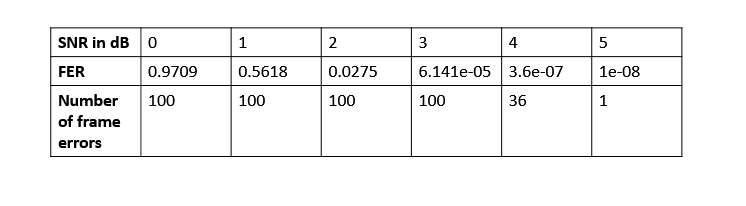
\includegraphics[width=0.8\textwidth]{FERTable.png}
	\caption{Data points from error plot simulation}
	\label{fig:ErrorTable}
\end{figure}
And the corresponding plot of the data points.
\begin{figure}[!htb]
	\setlength\fwidth{0.95\textwidth}
	\setlength\fheight{0.4\textheight}
	\centering
	% This file was created by matlab2tikz.
%
%The latest updates can be retrieved from
%  http://www.mathworks.com/matlabcentral/fileexchange/22022-matlab2tikz-matlab2tikz
%where you can also make suggestions and rate matlab2tikz.
%
\definecolor{mycolor1}{rgb}{0.00000,0.44700,0.74100}%
%
\begin{tikzpicture}

\begin{axis}[%
width=0.951\fwidth,
height=\fheight,
at={(0\fwidth,0\fheight)},
scale only axis,
xmin=0,
xmax=6,
ymode=log,
ymin=1e-14,
ymax=1,
yminorticks=true,
axis background/.style={fill=white},
xmajorgrids,
ymajorgrids,
yminorgrids,
legend style={legend cell align=left, align=left, draw=white!15!black}
]
\addplot [color=mycolor1]
  table[row sep=crcr]{%
0	0.970873786407765\\
0.207089034514839	0.886158625566635\\
0.396468066078011	0.808688202487994\\
0.569679094946515	0.737831721822905\\
0.72813012135502	0.673013204420059\\
0.873108145518025	0.613706169336469\\
1.00127616687936	0.561115893572658\\
1.09610418268403	0.51044904154491\\
1.18304919717487	0.463994097334841\\
1.2628092104682	0.421378117690295\\
1.3360212226702	0.382260751820979\\
1.40326723387787	0.346331035582549\\
1.46507624417937	0.313306322871293\\
1.52193025365504	0.282929079808215\\
1.57426426237738	0.254966884739035\\
1.62247227041204	0.229209222418269\\
1.66690727781788	0.205467484009224\\
1.70788728464788	0.183571761268081\\
1.74569329094888	0.163371915149203\\
1.78057429676238	0.144734904291862\\
1.81274730212455	0.127544785020248\\
1.84240030706672	0.111701108435497\\
1.86969531161589	0.0971173175077392\\
1.89476831579472	0.0837207470760979\\
1.91773431962239	0.0714499523354174\\
1.93868832311472	0.060254174533614\\
1.95770832628472	0.0500917380637132\\
1.97485532914255	0.0409300504638505\\
1.99018033169672	0.0327418622986965\\
2.00276133379356	0.0274194345219116\\
2.09336934889489	0.0249337142898253\\
2.17646736274456	0.0226540217698943\\
2.25272137545356	0.0205620860624786\\
2.32273838712307	0.0186412548611499\\
2.38707339784557	0.0168763024162082\\
2.4462294077049	0.0152534295346823\\
2.50066341677724	0.0137600989776301\\
2.55078942513157	0.0123849531587889\\
2.59697943282991	0.0111177867107924\\
2.63956743992791	0.00994943675003731\\
2.67885144647524	0.00887172800911728\\
2.71509645251608	0.00787739053547292\\
2.74853345808891	0.006960087125175\\
2.77936446322741	0.0061142761540085\\
2.80776346796058	0.00533518414368909\\
2.83387847231308	0.00461875089429681\\
2.85783547630591	0.00396151974914304\\
2.87973647995608	0.00336069246233697\\
2.89966848327808	0.00281388229473649\\
2.91770048628342	0.00231919631529779\\
2.93388648898108	0.00187515309972576\\
2.94827249137875	0.00148049069399123\\
2.96089249348208	0.00113427634946393\\
2.97177549529592	0.000835714486429805\\
2.98094549682425	0.000584146694091027\\
2.98842449807075	0.000378969429216247\\
2.99423549903925	0.000219551714790884\\
2.99840949973492	0.000105043103534383\\
3.00218250036375	6.12764303565223e-05\\
3.09314251552375	5.57233513308062e-05\\
3.17656152942692	5.06306479529896e-05\\
3.25310754218459	4.5957539035856e-05\\
3.32339155389859	4.16667232240329e-05\\
3.38796956466159	3.77242568946278e-05\\
3.44734757455793	3.40992489088213e-05\\
3.50198358366393	3.07637385125039e-05\\
3.55229359204893	2.76923290381879e-05\\
3.59865159977527	2.48621879050069e-05\\
3.64139360689894	2.22528024199898e-05\\
3.6808206134701	1.98457966290168e-05\\
3.71719661953277	1.76250534161821e-05\\
3.75075462512577	1.55763482057052e-05\\
3.78169863028311	1.3687226862568e-05\\
3.81020263503377	1.19470667421963e-05\\
3.83641763940294	1.03466493426894e-05\\
3.86046864341144	8.87834345386468e-06\\
3.88246064707677	7.53573885916866e-06\\
3.90247865041311	6.31364633567718e-06\\
3.92059365343228	5.2077313560065e-06\\
3.93686165614361	4.21457513799476e-06\\
3.95132665855444	3.33149149565766e-06\\
3.96402466067078	2.55628264046258e-06\\
3.97498466249744	1.88717813164721e-06\\
3.98423066403844	1.32271277685641e-06\\
3.99178466529744	8.61543483098054e-07\\
3.99766966627828	5.02266107698561e-07\\
4.00213566702261	3.59252516542086e-07\\
4.09498568249761	3.26755011125835e-07\\
4.18012769668795	2.96955306159217e-07\\
4.25824370970729	2.6961470160245e-07\\
4.32995872165979	2.44514447419074e-07\\
4.39584073264012	2.21455743575957e-07\\
4.45640674273446	2.0025764004294e-07\\
4.51212575202096	1.80755986792665e-07\\
4.56342476057079	1.62801333800222e-07\\
4.6106867684478	1.46259631043272e-07\\
4.65425677570946	1.31010128501688e-07\\
4.6944437824073	1.16944676157446e-07\\
4.73151978858663	1.03968073994679e-07\\
4.76572579428763	9.19959719993285e-08\\
4.7972717995453	8.09548701591452e-08\\
4.8263388043898	7.07814184635697e-08\\
4.8530838088473	6.14206669034443e-08\\
4.87763681293947	5.28271154711861e-08\\
4.90010781668464	4.49622641603774e-08\\
4.9205868200978	3.77946129657689e-08\\
4.93914682319114	3.12986118831018e-08\\
4.95584782597464	2.54532609088769e-08\\
4.97073682845614	2.02421100403517e-08\\
4.98385083064181	1.56522092753681e-08\\
4.99521983253664	1.16730586121765e-08\\
5.00215983369331	9.97840166306694e-09\\
5.09263084877181	9.07369151228193e-09\\
5.17560486260081	8.24395137399188e-09\\
5.25174587529098	7.48254124709022e-09\\
5.32166088694348	6.7833911305652e-09\\
5.38590189765032	6.14098102349683e-09\\
5.44497290749548	5.55027092504515e-09\\
5.49932891655482	5.00671083445181e-09\\
5.54938292489715	4.50617075102846e-09\\
5.59550793258466	4.04492067415345e-09\\
5.63803593967266	3.61964060327344e-09\\
5.67726594621099	3.2273405378901e-09\\
5.71345995224333	2.86540047756675e-09\\
5.74685095780849	2.53149042191506e-09\\
5.77763896293983	2.22361037060173e-09\\
5.80599696766616	1.94003032333839e-09\\
5.83207397201233	1.67926027987671e-09\\
5.855993975999	1.44006024001004e-09\\
5.8778609796435	1.22139020356504e-09\\
5.89775998296	1.02240017040002e-09\\
5.91575898595983	8.42410140401685e-10\\
5.93191398865233	6.80860113476686e-10\\
5.94626899104483	5.37310089551681e-10\\
5.95885899314317	4.11410068568348e-10\\
5.969711994952	3.02880050480008e-10\\
5.97885199647533	2.1148003524667e-10\\
5.986301997717	1.36980022830002e-10\\
5.99208399868067	7.9160013193338e-11\\
5.99622999937167	3.77000062833321e-11\\
5.99878899979817	1.21100020183373e-11\\
5.99988099998017	1.19000019833671e-12\\
5.99999899999983	1.00000016622914e-14\\
};
\addlegendentry{data1}

\end{axis}
\end{tikzpicture}%
	\caption{Plot of error floor calculation}
	\label{fig:ErrorFloor}
\end{figure}
As seen in the figure and more importantly the data points our error floor of $10^{-6}$ can be confirmed. As mentioned before a minimum number of frame errors are needed to confirm a \gls{FER}. While 36 frame errors are not the optimal number of errors it is still enough to validate an error floor of $10^{-6}$.






\clearpage

        %%%%%%%%%%%%%%%%%%%%%%%%%%%%%%%%%%%%%%%%%%%%%%%
\chapter{Summary} \label{chap:ending}
%%%%%%%%%%%%%%%%%%%%%%%%%%%%%%%%%%%%%%%%%%%%%%%
\graphicspath{{C:/Users/Kevin/Bachelarbeit/Bachelorarbeit/01_Bachelorarbeit_LaTex/02_Figures/}}
\section{AWGN vs. Rayleigh Comparison}
In this section a short summary between the two simulated channel is given. We will compare the methods and efficiency of both channels and relate it to real world applications. 
\part{title}

\begin{figure}[!htb]
    \centering
    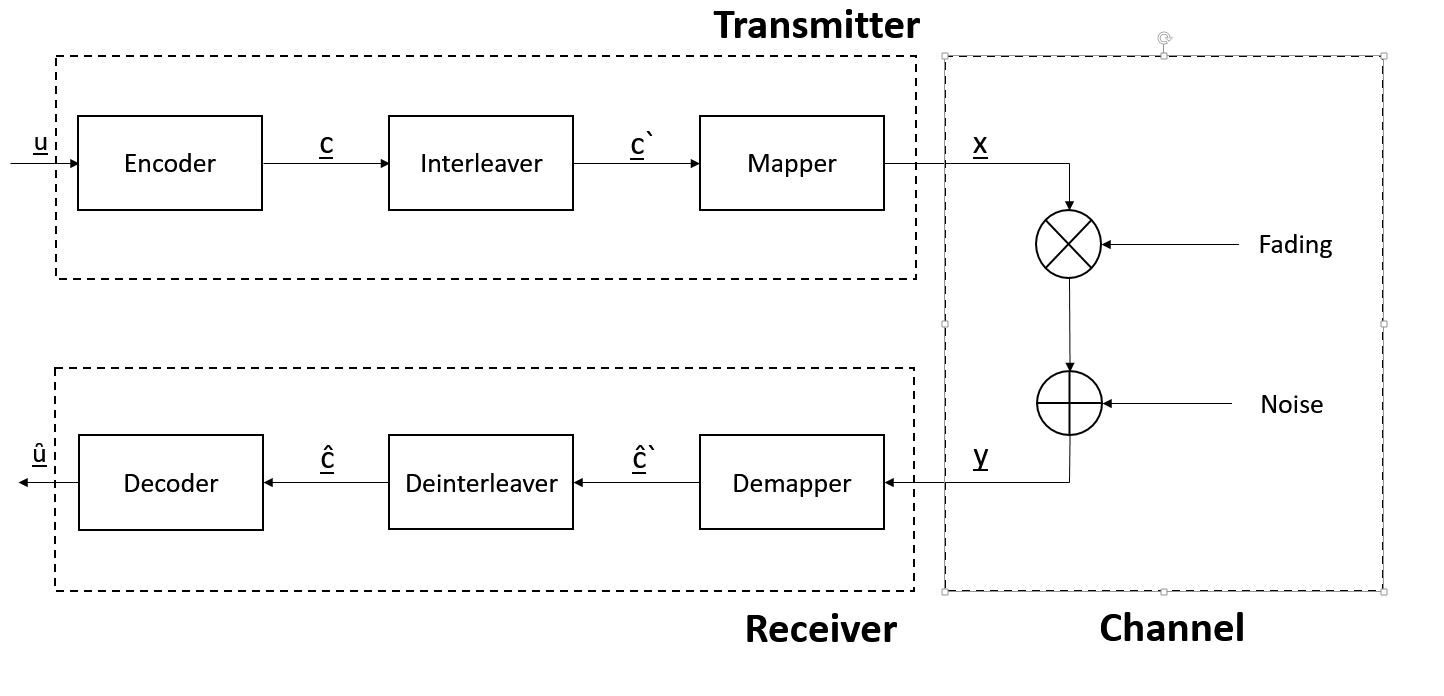
\includegraphics[width=0.8\textwidth]{Channelmodel.PNG}
    \caption{PDF $p_N(N)$ of the number N of times that the head side is up.}
    \label{fig:coin_bino}
\end{figure}



\clearpage

        %\include{...}          % Include ... / Einbinden des Kapitels ...
        %\include{simulation}   % Include simulation results / Einbinden des Kapitels Simulation
        %\include{conclusion}   % Include conclusion/summary / Einbinden des Kapitels Zusammenfassung/Ausblick
        
        \cleardoubleemptypage


% ########################################
% Appendix / Anhang:
% ########################################

% roman page numbering, starting with page number 1 (capitals)/ roemische Seitennummerierung beginnend mit Seite 1 (gross)
    \appendix
    \setcounter{page}{1}
    \pagenumbering{Roman}

        % Use IEEE DIN 1505 style for bibliography / Literaturverzeichnisses
        \bibliographystyle{IEEEtran}
        \nocite{*}              % Include all references without checking / Alle References immer aufführen
        \bibliography{citations}

\end{document}

%
% EOF!
%